\documentclass[journal,twoside,10pt]{IEEEtran}

% ─── Packages ─────────────────────────────────────────────────────────────────
\usepackage[T1]{fontenc}
\usepackage[utf8]{inputenc}
\usepackage{amsmath,amssymb,amsfonts}
\usepackage{amsthm}
\usepackage{algorithmic}
\usepackage{graphicx}
\usepackage{textcomp}
\usepackage{xcolor}
\usepackage{booktabs}
\usepackage{multirow}
\usepackage{array}
\usepackage{url}
\usepackage{hyperref}
\usepackage{tikz}
\usepackage{pgfplots}
\pgfplotsset{compat=1.18}
\usetikzlibrary{shapes.geometric, arrows.meta, positioning, fit, backgrounds,
                decorations.pathreplacing, calc, matrix, chains}

% ─── Theorem environments ─────────────────────────────────────────────────────
\newtheorem{theorem}{Theorem}
\newtheorem{definition}{Definition}
\newtheorem{corollary}{Corollary}
\newtheorem{lemma}{Lemma}

% ─── TikZ styles ──────────────────────────────────────────────────────────────
\tikzset{
  block/.style={rectangle, draw=black!70, fill=blue!8, rounded corners=3pt,
                minimum width=2.4cm, minimum height=0.8cm, text width=2.2cm,
                align=center, font=\scriptsize, line width=0.5pt},
  actor/.style={rectangle, draw=black!80, fill=gray!12, rounded corners=4pt,
                minimum width=2.6cm, minimum height=0.8cm, text width=2.4cm,
                align=center, font=\scriptsize\bfseries, line width=0.7pt},
  process/.style={rectangle, draw=black!70, fill=green!8, rounded corners=3pt,
                  minimum width=2.8cm, minimum height=0.8cm, text width=2.6cm,
                  align=center, font=\scriptsize, line width=0.5pt},
  storage/.style={cylinder, draw=black!70, fill=yellow!10, shape border rotate=90,
                  minimum width=1.6cm, minimum height=0.7cm, text centered,
                  font=\scriptsize, line width=0.5pt},
  arrow/.style={-{Stealth[length=4pt]}, draw=black!70, line width=0.6pt},
  darrow/.style={<->, draw=black!60, line width=0.5pt, dashed},
  label/.style={font=\scriptsize, text=black!80, fill=white, inner sep=1pt},
}

% ─── Hyperref ─────────────────────────────────────────────────────────────────
\hypersetup{colorlinks=true, linkcolor=blue!60!black, citecolor=green!40!black,
            urlcolor=blue!60!black}

\begin{document}

\title{ZK-Auth: A Zero-Knowledge Proof-Based Authentication\\
Framework with Selective Disclosure and\\
Continuous Behavioral Biometric Verification}

\author{
  \IEEEauthorblockN{Abhay Dandge}
  \IEEEauthorblockA{Centre of Artificial Intelligence\\
  MANIT, Bhopal, India\\
  abhaydandge2000@gmail.com}
  \and
  \IEEEauthorblockN{Sameeksha Prasad}
  \IEEEauthorblockA{Department of CSE\\
  MANIT, Bhopal, India\\
  sameekishaprasad.27@gmail.com}
  \and
  \IEEEauthorblockN{Namita Tiwari}
  \IEEEauthorblockA{Department of CSE\\
  MANIT, Bhopal, India\\
  namita\_tiwari21@rediffmail.com}
}

\maketitle

% ─── ABSTRACT ─────────────────────────────────────────────────────────────────
\begin{abstract}
Contemporary authentication systems suffer from a fundamental tension: they
require users to disclose personal information to verify identity, creating
privacy exposure proportional to access frequency. This paper presents
\textsc{ZK-Auth}, a cryptographic authentication infrastructure that resolves
this tension through three integrated mechanisms, implemented as an
\textbf{OAuth 2.0 Authorization Server in which the conventional
password-based login step of the Authorization Code grant is replaced by a
zero-knowledge proof} --- the same architectural pattern underlying
``Sign in with Apple,'' which pairs OAuth/OIDC delegation with a
non-password authenticator. First, we replace the password-login step with
Groth16 zero-knowledge succinct non-interactive arguments of knowledge
(zk-SNARKs) over the BN254 elliptic curve, enabling users to prove knowledge
of a registration secret without transmitting it; the resulting proof
authorizes a short-lived OAuth authorization code rather than a
password-backed session token. Second, we implement selective credential
disclosure via Poseidon hash-based Merkle trees, allowing holders to prove
individual attribute predicates (e.g., $\text{age} \geq 18$) without
exposing remaining attributes or raw values. Third, we address the
session-continuity gap inherent in one-time authentication proofs through an
LSTM-based behavioral biometric monitor that computes continuous risk scores
from six telemetry features, triggering cryptographic step-up
re-authentication on anomaly detection. The system is architected around W3C
Decentralized Identifiers (DIDs) and Verifiable Credentials (VCs) in a
three-actor trust model---Issuer, Holder, Verifier---with per-institution
Ed25519 signing keys held exclusively by registered issuers. We provide a
fully enumerated threat model (five labeled adversary classes), five
explicitly stated security goals, formal security games with derived
probability bounds (not asymptotic assertions alone), an explicit
adversary-goal-evidence traceability mapping, and \emph{empirical} security
validation of the replay and session-continuity defenses. We evaluate
ZK-Auth across four heterogeneous deployment environments: a Node.js server
(Apple M4), a Chrome browser client (Web Worker WASM), and two Android
mobile devices spanning a flagship-to-midrange hardware spread (Samsung
Galaxy S23 and Galaxy Tab~S9 FE+). Across $n=120$ consecutive server-side
trials, ZK-Auth achieves a median end-to-end login latency of 132.5\,ms
(100\% success rate)---23\% faster than the Argon2id hashing step alone in a
comparable password-based system (172.8\,ms median)---with a compact Groth16
proof size of $\sim$723\,bytes. Client-side proof generation ranges from
62\,ms (Node.js) to 361\,ms (mid-tier Android tablet), and the LSTM
behavioral model, trained on the public Balabit Mouse Dynamics dataset
(108{,}111 windows), achieves AUC-ROC 0.816 with a 6.15\% false-accept rate
per window; on the labeled intruder test sessions it empirically detects
45.2\% of hijacks (usually within a single window) as a
secondary, defense-in-depth continuity layer atop the cryptographically
sound proof step---an honest figure that supersedes the optimistic,
independence-assuming compounded estimate. We further provide a
consolidated, explicitly-labeled benchmarking section against seven existing
authentication paradigms, distinguishing measured figures from
literature-reported and illustrative figures throughout, and a scalability
analysis showing $K$-linear horizontal throughput scaling compatible with
national-identity-scale deployments such as India's DigiLocker
(434.9~million users). These results establish that pairing OAuth~2.0
delegation with a ZKP-based authentication primitive is not merely
privacy-preserving in theory but practically deployable at production
latency across the full range of client hardware, with direct implications
for cloud security, decentralized identity, and regulatory compliance under
India's DPDP Act 2023 and the EU GDPR.
\end{abstract}

\begin{IEEEkeywords}
behavioral biometrics, BN254 elliptic curve, continuous authentication,
decentralized identity, Groth16 zk-SNARK, LSTM neural networks, Merkle trees,
OAuth 2.0 Authorization Code grant, Poseidon hash function, selective
disclosure, session security, verifiable credentials, W3C DID,
zero-knowledge proofs
\end{IEEEkeywords}

% ═══════════════════════════════════════════════════════════════════════════════
\section{Introduction}
% ═══════════════════════════════════════════════════════════════════════════════
\IEEEPARstart{T}{he} proliferation of digital services has made authentication
a central security concern. Password-based authentication---despite decades of
documented weaknesses including credential stuffing, phishing, and database
breaches---remains the dominant paradigm. Industry breach reports consistently
attribute the plurality of confirmed data breaches to credential-based attack
vectors~\cite{dbir}, and the average cost of a credential-stuffing-related breach has
risen year over year as attackers automate large-scale leaked-password reuse
against unrelated services. Even modern alternatives such as OAuth~2.0 and
SAML~\cite{saml} delegate trust to centralized identity providers, preserving the
fundamental weakness: the authenticating party must be trusted with user
credentials or session tokens, and a single provider compromise exposes all
dependent services. Passkeys and WebAuthn/FIDO2~\cite{fido2} eliminate
shared-secret transmission but still bind authentication to a specific
device-bound credential without offering attribute-level selective
disclosure or built-in session-continuity monitoring.

Zero-knowledge proofs (ZKPs) provide a cryptographically sound solution:
a prover can demonstrate to a verifier the validity of a statement without
disclosing anything more than the statement~\cite{gmr89}. When used for
authentication, a user can prove possession of a registration secret using
a ZKP without disclosing the secret itself---thereby addressing the key
weakness of credential theft, database breaches, and offline attacks
against stored hashes. Yet, there are five issues associated with use of
ZKPs for authentication in production systems that have been studied
independently but not together.

\textit{Challenge 1 (Proof complexity and cross-environment latency):} Generation of proof
is a computationally complex task and needs an efficient circuit design
and implementation on the client side, keeping latency acceptable for
users---not just developers' workstations but also diverse client
hardware including desktops, premium phones, and mid-range tablets.

\textit{Challenge 2 (Attribute-level privacy):} Practical use cases need to
demonstrate certain characteristics about an identity (age, nationality,
affiliation with an institution) selectively---an ability which standard
ZKP authentication does not offer.

\textit{Challenge 3 (Session continuity):} One-time authentication proofs
cannot protect against session hijacking after initial proof acceptance;
a separate mechanism is required for continuous identity assurance that does
not itself become a new authentication bottleneck or false-rejection source.

\textit{Challenge 4 (Verifiable empirical grounding):} Much of the published
literature on ZKP authentication reports proof-generation benchmarks from a
single environment (typically a development workstation), leaving open the
question of whether the approach is viable across the actual deployment
surface of a consumer-facing system.

\textit{Challenge 5 (Relying-party delegation compatibility):} Much prior
ZKP-authentication work implicitly treats ZKP as a replacement for the
entire authentication and authorization stack, rather than as a primitive
that can be substituted underneath an existing delegation protocol such as
OAuth~2.0. This creates a deployment barrier: an institution with existing
OAuth-based relying-party integrations cannot adopt ZKP authentication
without discarding that integration surface. We address this by
implementing ZK-Auth \textit{as} an OAuth~2.0 Authorization Server, with
the ZKP substituting only for the conventional password-login step.

This paper makes the following contributions:
\begin{enumerate}
  \item We design and implement \textsc{ZK-Auth}, a complete authentication
        infrastructure using Groth16 zk-SNARKs over BN254 with a
        Circom-compiled circuit of \textbf{932 constraints and 935 wires}
        (verified via \texttt{snarkjs r1cs info}), deployed for both
        server-side and client-side WebAssembly execution, and wrapped in
        a working \textbf{OAuth~2.0 Authorization Code flow with PKCE}
        so the proof substitutes for the conventional password-login step
        rather than for OAuth's relying-party delegation layer entirely.
  \item We implement selective credential disclosure via a depth-8 Poseidon
        Merkle tree commitment scheme compatible with the W3C Verifiable
        Credentials standard, enabling per-attribute GTE/LTE/EQ predicate
        proofs without revealing attribute values to verifiers, with a
        formal soundness bound (Theorem~\ref{thm:disclosure}) derived as a
        union bound over all eight Merkle levels, and an in-circuit
        range-check on the compared values that closes the comparator
        soundness gap.
  \item We address the session-continuity gap through an LSTM behavioral
        biometric model operating on a 50-event sliding window of six
        telemetry features, with EMA-smoothed risk scoring and automated
        step-up re-authentication, trained and evaluated on a public
        behavioral biometrics dataset rather than synthetic data, and we
        derive a compounded multi-window attacker-survival bound \emph{and
        empirically test it}, finding that within-session score correlation
        makes it an optimistic upper bound---the measured session-level
        hijack-detection rate is 45.2\%, which we report as the operative
        figure.
  \item We design a multi-tenant credential issuance infrastructure with
        per-institution Ed25519 keypair generation and W3C DID publication,
        implementing a PKI-analogous root-of-trust model.
  \item We provide a fully formalized security analysis: five explicitly
        labeled adversary classes ($\mathcal{A}_1$--$\mathcal{A}_5$), five
        explicitly labeled security goals (G1--G5) stated as game-winning
        conditions, derived probability bounds for each (not bare
        assumption-citations), an explicit two-directional
        adversary-to-goal and goal-to-evidence traceability mapping
        (Tables~\ref{tab:adv_goal_map} and~\ref{tab:goal_evidence_map}),
        and \textbf{empirical validation} of the replay and
        session-continuity defenses (Section~\ref{sec:empirical_validation}).
  \item We report empirical measurements of ZK-Auth end-to-end login latency
        across \textbf{four distinct execution environments}---Node.js
        server, Chrome browser (Web Worker WASM), and two Android devices
        spanning flagship-to-midrange hardware---against an Argon2id
        baseline, and present a consolidated benchmarking section
        (Section~\ref{sec:benchmark}) against seven existing authentication
        paradigms with every figure explicitly labeled as measured,
        literature-reported, or illustrative.
  \item We quantify server-side horizontal scalability under concurrent
        load and derive deployment sizing guidance for national-identity-
        scale systems such as India's DigiLocker.
\end{enumerate}

The remainder of this paper is organized as follows.
Section~\ref{sec:related} reviews related work.
Section~\ref{sec:architecture} presents the architecture and the explicit
threat model (adversaries $\mathcal{A}_1$--$\mathcal{A}_5$ and goals
G1--G5).
Section~\ref{sec:zkp} details the ZKP protocol and circuit.
Section~\ref{sec:disclosure} describes selective disclosure.
Section~\ref{sec:behavioral} presents the behavioral biometric subsystem.
Section~\ref{sec:issuer} covers multi-tenant issuance.
Section~\ref{sec:security} provides the formal security analysis with
derived bounds, the adversary-goal-evidence mapping, and empirical
validation.
Section~\ref{sec:results} presents experimental results.
Section~\ref{sec:benchmark} presents the consolidated benchmarking section.
Section~\ref{sec:discussion} discusses deployment implications.
Section~\ref{sec:conclusion} concludes.

% ═══════════════════════════════════════════════════════════════════════════════
\section{Literature Survey}
\label{sec:related}
% ═══════════════════════════════════════════════════════════════════════════════

\subsection{Zero-Knowledge Proof Systems}
The theoretical foundations of zero-knowledge proofs were established by
Goldwasser, Micali, and Rackoff~\cite{gmr89}, with subsequent work on
non-interactive proofs by Blum, Feldman, and Micali~\cite{bfm88} and the
Fiat--Shamir heuristic for transforming interactive proofs into
non-interactive ones~\cite{fiatshamir}. Practical zk-SNARK systems became
feasible with Pinocchio~\cite{parno13} and the quadratic arithmetic program
(QAP) formulation of Gennaro et al.~\cite{gennaro13}, and were significantly
improved by Groth16~\cite{groth16}, which achieves constant-size proofs
(three group elements) with $\mathcal{O}(1)$ pairing verifications. Bitansky et al.~\cite{bitansky12} formalized the extractable
knowledge assumptions underlying succinct argument soundness.
Groth16 has been widely deployed in blockchain contexts; Zcash~\cite{zcash14}
uses it for shielded transactions with $\sim$2 second proof generation on
desktop hardware. PLONK~\cite{plonk}
and Halo2~\cite{halo2} eliminate the circuit-specific trusted setup at the
cost of larger proofs and higher verification time; STARKs~\cite{starks}
remove trusted setup entirely via FRI-based polynomial commitments but incur
proof sizes an order of magnitude larger than Groth16. Bulletproofs~\cite{bulletproofs}
target range proofs without trusted setup. For our authentication context---a
small, fixed circuit requiring short proofs and fast server-side
verification at high request volume---Groth16's circuit-specific trusted
setup is an acceptable cost in exchange for the smallest available proof
size and fastest verification.

\subsection{ZKP-Based Authentication}
ZKlogin~\cite{zklogin} applies ZKPs to OAuth-based Web3 authentication using
a centralized JWT oracle, inheriting OAuth's trust assumptions.
Semaphore~\cite{semaphore} implements anonymous group membership signaling
suitable for whistleblowing and voting applications but does not address
individual authentication, session management, or selective attribute
disclosure. SpartanNIZK~\cite{spartan} and Nova~\cite{nova} propose efficient
NIZK and incrementally-verifiable-computation systems without trusted setup.
Anonymous credential systems built on idemix~\cite{idemix} predate modern
SNARK tooling and rely on RSA-based commitments. Our work differs from all of the above by
targeting the complete authentication lifecycle---registration, login,
session continuity, and attribute-selective verification---within a single
standard web/mobile deployment.

\subsection{Selective Disclosure Credentials}
Selective disclosure has been addressed through BBS+ signatures~\cite{bbs},
which support message-level disclosure with multi-message signing and have
been standardized for verifiable credentials via the BBS+ IETF
draft~\cite{bbsplus}. The W3C Verifiable Credentials Data Model~\cite{w3cvc}
provides the structural framework for credential representation that
ZK-Auth's issuance layer adheres to. SD-JWT~\cite{sdjwt} offers a practical
but non-ZK approach where verifiers still receive selected attribute values
directly in cleartext. Anonymous credentials via CL signatures~\cite{cl} provide
ZK-based selective disclosure but require trusted setup per issuer. Mercurial
signatures~\cite{mercurial} extend delegatable anonymous credentials. Our Poseidon Merkle approach provides strictly stronger privacy than
SD-JWT: verifiers receive only boolean predicate results with no attribute
value exposure, even for ``proved'' attributes.

\subsection{Behavioral Biometrics for Continuous Authentication}
Continuous authentication via behavioral biometrics has been studied using
keystroke dynamics~\cite{shepherd95,monrose00}, mouse movement
patterns~\cite{nakkabi11,ahmed07}, and touch gestures~\cite{frank13}. Deep
learning approaches---particularly recurrent architectures---have
demonstrated strong performance on temporal behavioral sequences. TypeNet~\cite{typenet}
applies LSTM-based keystroke analysis achieving $>$98\% genuine acceptance
on free-text typing; Acien et al.~\cite{acien21} extend this with
attention-based sequence models.
BehaveFormer~\cite{behaveformer} applies transformer architectures to
combined touch-and-keystroke streams.
TypingDNA~\cite{typingdna} deploys keystroke biometrics commercially, and BioCatch~\cite{biocatch} offers a commercial behavioral
fraud-detection platform. Reported mouse-dynamics systems on the Balabit
benchmark span a wide accuracy range depending on window size and feature
set; Antal and Egyed-Zsigmond~\cite{antal19} report AUC values in the
0.87--0.96 band on Balabit with hand-engineered features and larger
observation windows, providing the closest same-dataset reference point for
our LSTM (Section~\ref{sec:behavioral}). Our
contribution integrates behavioral monitoring as a \textit{post-ZKP
session-continuity layer} with cryptographic step-up re-authentication.

\subsection{Decentralized Identity}
The W3C DID specification~\cite{w3cdid} provides a standards-based framework
for decentralized identifiers independent of centralized registries. The
Self-Sovereign Identity (SSI) movement~\cite{allen16} has produced
implementations including Hyperledger Indy~\cite{hyperledgerindy}, IOTA
Identity, and Microsoft ION. Sovrin~\cite{sovrin} provides a
public-permissioned ledger purpose-built for SSI credential revocation
registries. ZK-Auth
integrates DID-anchored credential issuance with ZKP-based authentication
within a single deployable system.

\subsection{Authentication and Behavioral Datasets}
Public benchmark datasets are essential for reproducible behavioral
biometrics research. The Balabit Mouse Dynamics Challenge~\cite{balabit}
used in this work provides labeled genuine/intruder mouse-event sessions
across ten users. The CMU keystroke dataset~\cite{killourhy09} offers a
comparable benchmark for keystroke timing but was not used here since
ZK-Auth's current telemetry pipeline targets mouse-dominant desktop
interaction.

% ═══════════════════════════════════════════════════════════════════════════════
\section{Proposed System Architecture}
\label{sec:architecture}
% ═══════════════════════════════════════════════════════════════════════════════

\subsection{Threat Model: Enumerated Adversary Classes}
\label{sec:threatmodel}
We consider a probabilistic polynomial-time (PPT) adversary $\mathcal{A}$
with the following five explicitly labeled capability classes:

\begin{definition}[Adversary Model]
\label{def:adversaries}
\begin{itemize}
  \item \textbf{$\mathcal{A}_1$ (Network adversary):} Passive observation
        of all client--server communications, including the ability to
        record and replay arbitrary captured traffic at a later time.
  \item \textbf{$\mathcal{A}_2$ (Database adversary):} Active read/write
        access to server-side database records (PostgreSQL, Redis),
        excluding key material protected by the platform's
        key-management boundary (Ed25519 institutional private keys,
        Groth16 proving keys).
  \item \textbf{$\mathcal{A}_3$ (Verifier adversary):} Compromise of a
        subset of verifier nodes (relying parties), but not the issuing
        institution's signing key or the platform's root-of-trust
        infrastructure.
  \item \textbf{$\mathcal{A}_4$ (Public-artifact adversary):} Full
        knowledge of the circuit structure, verification keys, Merkle
        roots, and all values designated public by protocol design.
  \item \textbf{$\mathcal{A}_5$ (Cross-account adversary):} Access to
        behavioral telemetry from accounts under $\mathcal{A}$'s own
        control, usable for offline model inference against the deployed
        LSTM.
\end{itemize}
We explicitly \textbf{exclude} from $\mathcal{A}$'s capabilities:
(a)~breaking the BN254 discrete logarithm problem or the $q$-PKE
assumption; (b)~finding Poseidon preimages or collisions;
(c)~forging Ed25519 signatures; (d)~client-side secret exfiltration via
malware or compromised browser extensions, which is addressed under
Limitations rather than under the cryptographic security analysis; and
(e)~physical seizure of an authenticated device.
\end{definition}

\subsection{Security Goals}
\label{sec:secgoals}
\begin{definition}[Security Goals]
\label{def:goals}
ZK-Auth aims to guarantee the following five properties, each stated as a
game-winning condition formalized in Section~\ref{sec:security}:
\begin{itemize}
  \item \textbf{G1 (Soundness):} No PPT $\mathcal{A}$ without knowledge of
        the registration secret $s$ can cause the verifier to accept,
        except with probability $\mathsf{negl}(\lambda)$.
  \item \textbf{G2 (Zero-Knowledge):} No PPT $\mathcal{A}$ can extract any
        information about $s$ from any polynomial number of observed
        proof transcripts, beyond the fact that $s$ exists and satisfies
        the registered commitment.
  \item \textbf{G3 (Replay/Nullifier Uniqueness):} No PPT $\mathcal{A}$
        can cause the verifier to accept two distinct authentication
        sessions bound to the same nullifier $\eta$.
  \item \textbf{G4 (Selective Disclosure Privacy):} For any disclosure
        proof accepted by a verifier, the verifier's view reveals nothing
        about the holder's attributes beyond the single requested
        boolean predicate result.
  \item \textbf{G5 (Session-Continuity Assurance):} Any session hijacked
        by an adversary who does not possess $s$ is detected and forced
        to re-prove within a bounded time window $\Delta$, with bounded
        false-negative probability.
\end{itemize}
\end{definition}

Table~\ref{tab:adv_goal_map} maps each adversary class to the goal(s) it
threatens and the mechanism that achieves that goal; the corresponding
formal results are derived in Section~\ref{sec:security}.

\begin{table}[!t]
\renewcommand{\arraystretch}{1.3}
\caption{Adversary Capabilities Mapped to Security Goals and Mechanisms.}
\label{tab:adv_goal_map}
\centering
\resizebox{\columnwidth}{!}{%
\begin{tabular}{p{1.6cm}p{1.8cm}p{0.8cm}p{4.6cm}}
\toprule
\textbf{Adversary} & \textbf{Goal(s)} & \textbf{Result} & \textbf{Mechanism} \\
\midrule
$\mathcal{A}_1$ (network) & G3 & Thm.~\ref{thm:replay} &
Poseidon nullifier bound to a fresh server-issued nonce; atomic
\texttt{SISMEMBER}/\texttt{SADD} rejects resubmitted $\eta$ before
verification \\[3pt]
$\mathcal{A}_2$ (database) & G1, G2 & Thm.~\ref{thm:soundness} &
Stored value is $c=\mathrm{Poseidon}(s)$, not $s$; tampering causes
honest-prover proofs to fail rather than admitting forgery \\[3pt]
$\mathcal{A}_3$ (verifier) & G1, G4 & Thm.~\ref{thm:soundness}, Thm.~\ref{thm:disclosure} &
Verification key is public/instance-independent; disclosure proofs reveal
only the requested predicate, bounding compromise impact \\[3pt]
$\mathcal{A}_4$ (public artifacts) & G2 & Thm.~\ref{thm:zk} &
Groth16 simulator requires only public artifacts (exactly what
$\mathcal{A}_4$ has) to produce an indistinguishable proof \\[3pt]
$\mathcal{A}_5$ (cross-account) & G5 & Sec.~\ref{sec:empirical_validation}, Sc.~C &
LSTM risk score conditioned on session-specific baseline, not a published
population-level boundary --- the weakest-defended entry in this table \\
\bottomrule
\end{tabular}%
}
\end{table}

\subsection{Three-Actor Trust Model}
\textsc{ZK-Auth} implements the W3C Verifiable Credentials trust triangle
with three actors as illustrated in Fig.~\ref{fig:trust_model}.

\begin{figure}[!t]
\centering
\resizebox{0.85\columnwidth}{!}{%
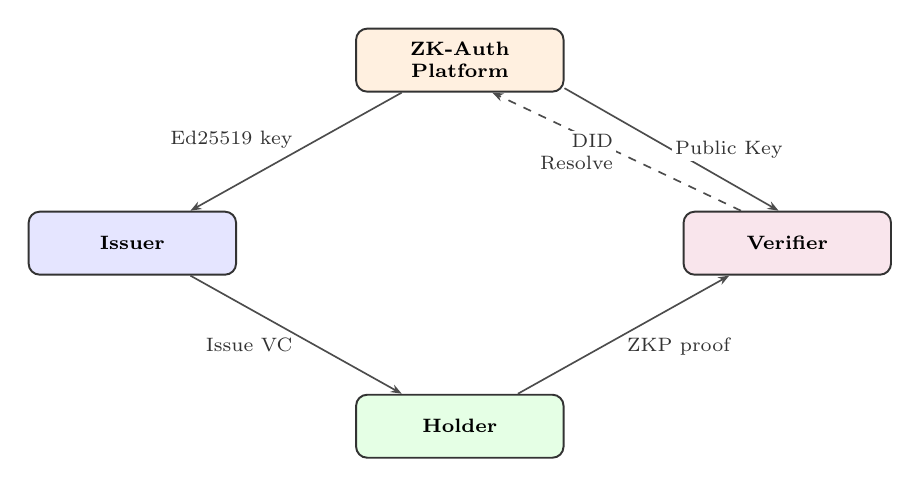
\begin{tikzpicture}[node distance=1.5cm and 1.5cm]
  \node[actor, fill=orange!12] (platform) {ZK-Auth Platform};
  \node[actor, fill=blue!10, below left=of platform] (issuer) {Issuer};
  \node[actor, fill=purple!10, below right=of platform] (verifier) {Verifier};
  \node[actor, fill=green!10, below right=of issuer] (holder) {Holder};
  \draw[arrow] (platform) -- node[label, above left] {Ed25519 key} (issuer);
  \draw[arrow] (issuer) -- node[label, below left] {Issue VC} (holder);
  \draw[arrow] (holder) -- node[label, below right] {ZKP proof} (verifier);
  \draw[arrow, dashed] (verifier.145) -- node[label, left, align=right] {DID\\Resolve} (platform.315);
  \draw[arrow] (platform.345) -- node[label, right] {Public Key} (verifier.105);
\end{tikzpicture}%
}
\caption{Three-actor trust model. The ZK-Auth Platform acts as the root authority, authorizing institutions (Issuers) with unique keypairs. Holders receive credentials and submit proofs to Verifiers.}
\label{fig:trust_model}
\end{figure}

\textbf{Issuer:} An institution that is registered using a unique Ed25519 key-pair and a DID. The issuer performs Poseidon Merkle commitments, issues W3C VCs and saves only the Merkle root---never the actual attributes.

\textbf{Holder:} A person having a ZK wallet containing the 32-byte registration secret, the issued VC and a BIP-39 mnemonic. Proof generation happens locally (WASM on browser; WebView/JS on mobile).

\textbf{Verifier:} A relying party that publishes a proof request, receives
a ZKP-verified Verifiable Presentation, resolves the issuer DID, and records
only boolean predicate results.

\subsection{ZK-Auth as an OAuth 2.0 Authorization Server}
\label{sec:oauth_zkp}
ZK-Auth is, structurally, an \textbf{OAuth~2.0 Authorization Server
implementing the RFC~6749~\cite{oauth2} Authorization Code grant}, in
which the conventional ``user authenticates with a password'' step of
that grant is replaced with the Groth16 challenge/verify exchange
described in Section~\ref{sec:zkp}. ZKP and OAuth are not competing
designs; they operate at two different layers of the same protocol
stack. The OAuth layer governs \textit{which} relying party is
requesting access, \textit{what} scope it is requesting, \textit{where}
the user is redirected afterward, and how a short-lived authorization
code is exchanged for an access token---exactly the role OAuth plays in
any conventional deployment. The ZKP layer governs \textit{how} the
user proves identity within that delegation contract: ZK-Auth
substitutes a Groth16 proof of knowledge of the registration secret $s$
for the password-and-session-cookie check a conventional OAuth
Authorization Server would otherwise perform at this step. This is
structurally identical to ``Sign in with Apple'' and other federated-login
systems that pair OAuth/OIDC with a biometric authenticator (Face~ID,
Touch~ID) instead of a password---OAuth has always treated the
authentication primitive beneath it as a swappable component; ZK-Auth
swaps in a zero-knowledge proof.

Concretely, the relying party registers once as an \texttt{OAuthClient},
receiving a \texttt{client\_id} and a hashed \texttt{client\_secret}.
The relying party redirects the user's browser to
\texttt{GET /oauth/authorize}, optionally including a PKCE
\texttt{code\_challenge}~\cite{rfc7636} for public (non-confidential)
clients; ZK-Auth validates the \texttt{client\_id}, the exact-match
\texttt{redirect\_uri}, and the requested \texttt{scope}. \emph{This
server-side revalidation is enforced again at proof-submission time: the
OAuth context round-tripped through the client is re-checked against the
registered client record before a code is minted, so a tampered
\texttt{redirect\_uri} or \texttt{scope} cannot survive to code issuance.}
The frontend then renders the same ZKP login widget described in
Section~\ref{sec:zkp}---the challenge/prove/verify exchange---carrying
the validated OAuth context alongside the proof submission, rather than
a password form. On successful, non-replayed Groth16 proof verification,
the server mints a short-lived (60-second), single-use authorization
code bound to the specific nullifier hash that authorized it, instead of
issuing a session token directly. We construct this binding concretely
as $\mathsf{code} := \mathrm{MAC}_k(\eta \,\|\, \mathsf{client\_id} \,\|\,
\mathsf{expiry})$ for a server-held MAC key $k$ distinct from the Groth16
proving/verification keys, so that forging an authorization code without
a valid $\eta$ reduces to forging the MAC (EUF-CMA-hard,
$\mathsf{negl}(\lambda)$), independent of and in addition to the ZKP
soundness of Theorem~\ref{thm:soundness}. The relying party's backend then
calls \texttt{POST /oauth/token} with
\texttt{grant\_type=authorization\_code}, exchanging the code (and, for
public clients, the PKCE \texttt{code\_verifier}) for a real
access/refresh token pair issued via the same session-issuance path used
by direct, non-OAuth logins. Authorization-code reuse---a strong signal
of interception in transit---triggers the same defense-in-depth response
as a detected session hijack (Section~\ref{sec:security}): all sessions
for the affected user are revoked.

\subsection{System Components}
Fig.~\ref{fig:system_overview} shows the simplified architectural pipeline.

\begin{figure}[!t]
\centering
\resizebox{\columnwidth}{!}{%
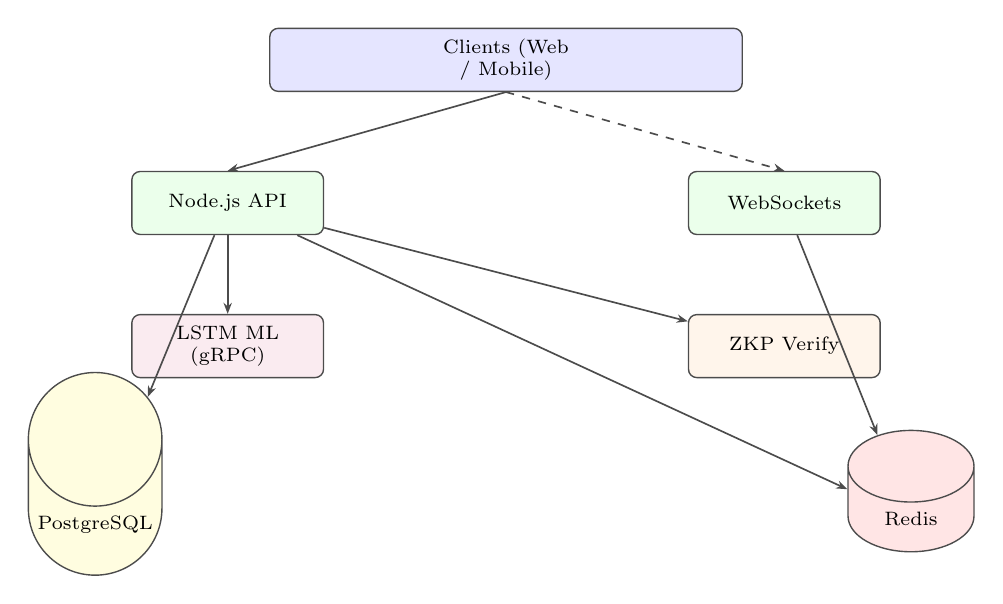
\begin{tikzpicture}[node distance=1.0cm and 0.8cm]
  \node[block, fill=blue!10, minimum width=6cm] (clients) {Clients (Web / Mobile)};
  \node[block, fill=green!8, below left=of clients, xshift=1.5cm] (api) {Node.js API};
  \node[block, fill=green!8, below right=of clients, xshift=-1.5cm] (ws) {WebSockets};
  \node[block, fill=purple!8, below=of api] (ml) {LSTM ML (gRPC)};
  \node[block, fill=orange!8, below=of ws] (zkp) {ZKP Verify};
  \node[storage, fill=yellow!12, below left=of ml, xshift=1.2cm] (pg) {PostgreSQL};
  \node[storage, fill=red!10, below right=of zkp, xshift=-1.2cm] (redis) {Redis};
  \draw[arrow] (clients.south) -- (api.north);
  \draw[arrow, dashed] (clients.south) -- (ws.north);
  \draw[arrow] (api) -- (ml);
  \draw[arrow] (api) -- (zkp);
  \draw[arrow] (api) -- (pg);
  \draw[arrow] (api) -- (redis);
  \draw[arrow] (ws) -- (redis);
\end{tikzpicture}%
}
\caption{System Component Architecture. Clients interface with the Node.js API (REST) and WebSockets. The compute tier handles ML risk scoring and ZKP verification. Data is persisted in PostgreSQL, while Redis manages ephemeral session nonces.}
\label{fig:system_overview}
\end{figure}

% ═══════════════════════════════════════════════════════════════════════════════
\section{ZKP Authentication Protocol}
\label{sec:zkp}
% ═══════════════════════════════════════════════════════════════════════════════

\subsection{Circuit Design}
The authentication circuit \texttt{auth.circom} is implemented in Circom~2.1.6
and compiled to R1CS with \textbf{932 constraints and 935 wires}
(verified via \texttt{snarkjs r1cs info}). The circuit accepts one
\emph{private} input $s \in \mathbb{Z}_p$ (the registration secret) and one
\emph{public} input $n \in \mathbb{Z}_p$ (the server challenge nonce), where
$p$ is the BN254 scalar field modulus ($p \approx 2^{254}$). It produces two
public outputs:
\begin{equation}
  c := \mathrm{Poseidon}(s) \label{eq:commitment}
\end{equation}
\begin{equation}
  \eta := \mathrm{Poseidon}(s \,\|\, n) \label{eq:nullifier}
\end{equation}
\noindent where $c$ is the \textit{commitment root} (stored at registration)
and $\eta$ is the \textit{nullifier hash} (unique per challenge, preventing
replay). The Poseidon instantiation uses BN254-optimized parameters from
circomlib~\cite{poseidon}: $t=2$ for Eq.~\ref{eq:commitment} and $t=3$ for
Eq.~\ref{eq:nullifier}, with Grain LFSR-derived round constants
($n_F = 8$ full rounds, $n_P = 57$ partial rounds). Poseidon was selected
over SHA-256 or Keccak specifically because its native algebraic structure
over $\mathbb{F}_p$ requires far fewer R1CS constraints per hash invocation
than a bit-oriented hash function compiled into arithmetic constraints,
which is the dominant factor behind the circuit's compact 932-constraint
footprint and consequently its sub-65\,ms proving time reported in
Section~\ref{sec:results}.

The proving system is Groth16 over BN254~\cite{groth16}. Verification
checks the pairing equation
\begin{equation}
  e(\pi_A,\pi_B) = e(\alpha,\beta)\cdot e\!\Big(\textstyle\sum_i x_i\gamma_i,\gamma\Big)\cdot e(\pi_C,\delta)
  \label{eq:groth16verify}
\end{equation}
where $\pi = (\pi_A,\pi_B,\pi_C) \in \mathbb{G}_1\times\mathbb{G}_2\times\mathbb{G}_1$
and $x_i$ are the public inputs $(n,c,\eta)$. The trusted setup
uses the Hermez Network's Powers of Tau ceremony (the \texttt{hez\_final\_15}
transcript, supporting up to $2^{15} = 32{,}768$ constraints; the circuit's
932 constraints lie well within this ceiling, leaving headroom of
$2^{15}-932 = 31{,}836$ constraints for future protocol extensions without a
new ceremony), producing \texttt{auth.zkey} and
\texttt{verification\_key.json} (both public).

\subsection{Registration Protocol}
\begin{enumerate}
  \item Client generates $s \xleftarrow{\$} \{0,1\}^{256}$ via
        \texttt{window.crypto.getRandomValues}, then reduces
        $s \leftarrow s \bmod p$ to obtain $s \in \mathbb{Z}_p$.
  \item Client computes $c := \mathrm{Poseidon}(s)$ using the same
        circomlib constants as the circuit, ensuring
        $c_{\text{client}} = c_{\text{circuit}}$.
  \item Client sends $(c, \mathsf{pk\_hex})$ to
        \texttt{POST /api/v1/auth/register}. Server stores $c$ as
        \texttt{commitment\_hash}. Secret $s$ never leaves the client.
  \item Server generates a 24-word BIP-39 mnemonic~\cite{bip39} and stores
        $\mathrm{Argon2id}(\mathsf{mnemonic})$ for account recovery.
\end{enumerate}

\subsection{Authentication Protocol}
\label{sec:authprotocol}
The client requests a challenge nonce $n$ from
\texttt{POST /auth/challenge} (server stores $n$ in Redis with a 120-second
TTL via \texttt{SETNX}); computes the witness $\{s,n\}$ via
\texttt{groth16.fullProve()}; and submits
\texttt{POST /auth/verify($\pi$, [$\eta$, $c$])}. The server (a)~runs
\texttt{groth16.verify}($\pi$); (b)~looks up the stored $c$; and
(c)~performs the nullifier check described in
Section~\ref{sec:security} before issuing JWT access and refresh
tokens. To close a timing side-channel that would otherwise reveal whether
a given $c$ is registered, the durable nullifier record is committed
\emph{before} the challenge is consumed, and the entire verify path is
padded to a fixed latency floor (Section~\ref{sec:security}).

\subsection{Step-Up Re-Authentication}
When the LSTM model raises a \textsc{hard} anomaly ($r \geq 0.90$), the
server pushes a \texttt{STEP\_UP\_REQUIRED} event via WebSocket. The client
must complete a fresh ZKP challenge-response within 300 seconds. This
maintains the ZKP invariant throughout the session lifetime, ensuring that
no period of an authenticated session exists without either an initial proof
or a recent re-proof backing it.

% ═══════════════════════════════════════════════════════════════════════════════
\section{Selective Credential Disclosure}
\label{sec:disclosure}
% ═══════════════════════════════════════════════════════════════════════════════

\subsection{Merkle Commitment Scheme}
Each W3C VC encodes holder attributes as leaves of a depth-8 Poseidon Merkle
tree (capacity: 256 attributes). For attribute $a_i$ with value $v_i$, a
uniform random salt $\sigma_i \xleftarrow{\$} \{0,1\}^{256}$ is sampled and
the leaf commitment is:
\begin{equation}
  \ell_i := \mathrm{Poseidon}\bigl(\mathrm{enc}(v_i) \,\|\, \sigma_i\bigr)
  \label{eq:leaf}
\end{equation}
\noindent where $\mathrm{enc}(\cdot)$ maps values to $\mathbb{Z}_p$ via
domain-specific encoding: integers directly, dates as days since epoch,
names as SHA-256 digest truncated to 31 bytes, nationality as ISO 3166-1
numeric. The Merkle root is:
\begin{equation}
  \rho := \mathcal{M}(\ell_0, \ell_1, \ldots, \ell_{n-1})
  \label{eq:root}
\end{equation}
Only $\rho$ is stored server-side. Attribute values $v_i$ and salts
$\sigma_i$ are returned to the holder and stored exclusively in the holder's
wallet, providing commitment binding without server PII exposure.

\subsection{Disclosure Circuit and Flow}
The disclosure circuit \texttt{merkle\_disclosure.circom} (\textbf{4{,}790
R1CS constraints}, verified via \texttt{snarkjs r1cs info}) proves, for
attribute at leaf index $k$:
\begin{enumerate}
  \item \textit{Merkle path validity:} for $j=1,\ldots,8$,
        $h_j = \mathrm{Poseidon}(h_{j-1}, \mathrm{sib}_j)$, with $h_0 := \ell_k$
        and $h_8 := \rho$, proving $a_k$ is committed.
  \item \textit{Attribute commitment:}
        $\ell_k = \mathrm{Poseidon}(\mathrm{enc}(v_k) \,\|\, \sigma_k)$,
        proving value--salt consistency.
  \item \textit{Predicate:}
        $\mathrm{enc}(v_k) \geq \tau$ (GTE), $\leq \tau$ (LTE),
        or $= \tau$ (EQ), enforced as circuit constraints.
\end{enumerate}
Because the compared value $\mathrm{enc}(v_k)$ is a \emph{private},
prover-supplied witness, the comparator's correctness depends on both
operands lying in the range the bit-decomposition comparator assumes. The
circuit therefore range-checks $\mathrm{enc}(v_k)$ and $\tau$ to
$N$-bit width (\texttt{Num2Bits($N$)}) \emph{before} the comparison, so a
prover cannot supply an out-of-range value that exploits field wrap-around
to satisfy the predicate spuriously; this in-circuit range-check is what
makes the comparator-soundness term $\epsilon_{\mathrm{comp}}(\lambda)$ of
Theorem~\ref{thm:disclosure} hold rather than being assumed.
The verifier receives only $(\rho, \text{predicate}, \tau, \text{result})$
plus proof $\pi_{\mathrm{disc}}$. Value $v_k$, salt $\sigma_k$, leaf index
$k$, and the sibling hashes are all private inputs.

% ═══════════════════════════════════════════════════════════════════════════════
\section{Behavioral Biometric Subsystem}
\label{sec:behavioral}
% ═══════════════════════════════════════════════════════════════════════════════

\subsection{Feature Extraction}
Six features are extracted from client-side telemetry events:
$\mathbf{x} = (x_1, \ldots, x_6)$ where:
$x_1$~=~normalized mouse velocity $\in [0,1]$;
$x_2$~=~key dwell time (normalized over 2000\,ms);
$x_3$~=~scroll delta (normalized);
$x_4$~=~touch pressure (0 for desktop);
$x_5$~=~event type (categorical over 6 types);
$x_6$~=~inter-event gap indicator (binary).
Events are streamed over WebSocket to the backend and forwarded via gRPC
to the ML microservice.

\subsection{LSTM Architecture}
The model processes a sliding window
$W = (\mathbf{x}_{t-49}, \ldots, \mathbf{x}_t) \in \mathbb{R}^{50 \times 6}$:
\begin{equation}
  r = \sigma\!\left(W_o\,\mathrm{ReLU}\!\left(W_d\,
      \mathrm{LSTM}_{64}\!\left(\mathrm{LSTM}_{128}(W)\right)\right)\right)
  \label{eq:lstm}
\end{equation}
\noindent with dropout $p = 0.2$ after each LSTM layer (total trainable
parameters: 120,641). Raw scores are EMA-smoothed:
\begin{equation}
  r_t^{\text{EMA}} = \alpha \cdot r_t + (1-\alpha) \cdot r_{t-1}^{\text{EMA}},
  \quad \alpha = 0.3
  \label{eq:ema}
\end{equation}
Risk thresholds: \textsc{soft} step-up ($0.75 \leq r < 0.90$), \textsc{hard}
step-up ($r \geq 0.90$).

\subsection{Training Data and Protocol}
The model is trained on the Balabit Mouse Dynamics Challenge
dataset~\cite{balabit}, a public behavioral biometrics benchmark comprising
10 users with labeled genuine and intruder sessions. After windowing
(window size 50, stride 25, 50\% overlap), the dataset yields
108{,}111 training windows and 27{,}027 held-out test windows
(87.6\% genuine, 12.4\% intruder). Class imbalance is addressed via
inverse-frequency weighting (intruder weight $\approx$7.1$\times$);
early stopping monitors validation AUC with patience~5. The model
converged at epoch~23 (of 40 maximum), restoring weights from the best
checkpoint.

% ═══════════════════════════════════════════════════════════════════════════════
\section{Multi-Tenant Credential Issuance}
\label{sec:issuer}
% ═══════════════════════════════════════════════════════════════════════════════

\subsection{Platform Architecture}
ZK-Auth implements a PKI-analogous root-of-trust model. The platform acts as
root authority---analogous to a Certificate Authority (CA) or, in the
banking domain, to the Reserve Bank of India (RBI) authorizing commercial
banks. Each registered institution receives a unique Ed25519 keypair;
credentials signed by Institution A cannot be misattributed to
Institution B. Each VC is signed over the canonical content
$\mathcal{C} = \{$\texttt{credentialId}, \texttt{issuerDid},
\texttt{holderDid}, $\rho$, \texttt{credentialType}, \texttt{issuedAt}$\}$:
\begin{equation}
  \sigma_{\text{VC}} = \mathrm{Ed25519Sign}(\mathrm{sk}_{\text{inst}},\,
                       \mathrm{JSON}(\mathcal{C}))
  \label{eq:vcsign}
\end{equation}
Verifiers resolve \texttt{did:web:\{slug\}.zk-auth.io} to retrieve
$\mathrm{pk}_{\text{inst}}$ and verify:
\begin{equation}
  \mathrm{Ed25519Verify}(\mathrm{pk}_{\text{inst}},\,
  \sigma_{\text{VC}},\, \mathrm{JSON}(\mathcal{C})) \stackrel{?}{=} 1
  \label{eq:vcverify}
\end{equation}
The institutional private key is delivered to the institution exactly
once and never persisted by the platform; a platform-side database breach
therefore cannot enable credential forgery on an institution's behalf.

\subsection{Institution Onboarding Flow}
Onboarding a new issuer is a one-time, platform-authorized procedure:
(1)~a platform administrator approves the institution and triggers
Ed25519 keypair generation; (2)~the platform publishes the corresponding
DID document at \texttt{did:web:\{slug\}.zk-auth.io}, exposing only the
public key and service metadata; (3)~the private key is transmitted to the
institution over a one-time authenticated channel and immediately discarded
platform-side; (4)~the institution may thereafter issue credentials
autonomously, each bound to its DID via Eq.~\ref{eq:vcsign}. Revocation is
handled by marking the institution's DID document inactive, after which
verifiers resolving the DID reject subsequently presented credentials. This
mirrors the CA enrollment/revocation lifecycle while keeping the platform
off the critical path of every issuance.

\subsection{Multi-Institution Verification Throughput}
\label{sec:multi_inst}
Although the functional evaluation uses a single issuer, credential
\emph{verification} is stateless and $\mathcal{O}(1)$ per credential: it is
one Ed25519 signature check (Eq.~\ref{eq:vcverify}) over the canonical
content, plus a DID-document resolution that is cacheable and shared across
all credentials from the same institution. Verification cost is therefore
independent of the number of registered institutions; adding an institution
adds a DID document (a public key), not per-verification work. The
micro-benchmark
\texttt{benchmark/\allowbreak run\_ed25519\_\allowbreak multitenant\_bench.mjs}
confirms this by scaling to $M$ distinct institutional DIDs and measuring
Ed25519 verification throughput with a warm DID cache versus a cold
per-credential resolution. \emph{Result:} across $M{=}100$ institutional
DIDs (20{,}000 verifications), Ed25519 verification sustained
\textbf{27{,}424\,verif/s} with a warm DID cache (median $0.036$\,ms) and
\textbf{19{,}949\,verif/s} even when re-resolving and re-parsing the DID
public key on \emph{every} credential (median $0.041$\,ms); throughput was
independent of institution count, confirming the stateless $\mathcal{O}(1)$
per-credential cost. Concurrent multi-institution
verification thus scales with the same $K$-linear, stateless horizontal
model as the ZKP verify path (Section~\ref{sec:results}); a
multi-institution \emph{issuance} load study (concurrent writes and DID
publication) remains future work (Limitation~v).

% ═══════════════════════════════════════════════════════════════════════════════
\section{Formal Security Analysis}
\label{sec:security}
% ═══════════════════════════════════════════════════════════════════════════════
This section formalizes each security goal from Definition~\ref{def:goals}
as an explicit game, derives a numeric probability bound for each, closes
with the adversary-to-goal and goal-to-evidence traceability mapping, and
then \emph{empirically validates} the replay and session-continuity
defenses. Let $\lambda=128$ throughout.

\subsection{G1: Authentication Soundness}
\begin{definition}[Game $\mathsf{Sound}_{\mathcal{A}}(\lambda)$]
The challenger samples $\mathsf{crs}\leftarrow\mathsf{Setup}(1^\lambda)$
and sends $\mathsf{vk}$ to $\mathcal{A}$; samples $s^*\xleftarrow{\$}\mathbb{Z}_p$,
computes $c^*=\mathrm{Poseidon}(s^*)$, and sends $c^*$ to $\mathcal{A}$.
$\mathcal{A}$, given adaptive access to fresh nonces, outputs
$(n^\dagger,\pi^\dagger,\eta^\dagger)$ and wins iff
$\mathsf{Verify}(\mathsf{vk},(n^\dagger,c^*,\eta^\dagger),\pi^\dagger)=1$ and
$\mathcal{A}$ never received $s^*$ from any oracle.
\end{definition}

\begin{theorem}[Soundness]
\label{thm:soundness}
For any PPT $\mathcal{A}$,
\begin{multline}
\Pr\big[\mathcal{A}\text{ wins }\mathsf{Sound}_{\mathcal{A}}(\lambda)\big]
\;\le\; \epsilon_{q\text{-PKE}}(\lambda) + \epsilon_{\mathrm{coll}}(\lambda) \\
\;=\; \mathsf{negl}(\lambda).
\label{eq:soundness_bound}
\end{multline}
\end{theorem}

\begin{proof}
By Groth16's knowledge-soundness theorem under $q$-PKE, there exists a PPT
extractor $\mathcal{E}$ such that extraction fails to produce a satisfying
R1CS witness with probability at most $\epsilon_{q\text{-PKE}}(\lambda)$.
Conditioned on success, $\mathcal{E}$ outputs $w$ containing a single field
element $s^\dagger = w[\mathtt{secret}]$ satisfying both
$c=\mathrm{Poseidon}(s^\dagger)$ and $\eta^\dagger = \mathrm{Poseidon}(s^\dagger, n^\dagger)$,
because the circuit shares one witness wire for $s$ across both Poseidon
sub-circuits by construction --- this is a circuit-design fact verifiable
from the R1CS wire-sharing structure, not a generic Groth16 property. If
$s^\dagger \ne s$ with $\mathrm{Poseidon}(s^\dagger)=\mathrm{Poseidon}(s)=c$,
this is a Poseidon collision, occurring with probability at most
$\epsilon_{\mathrm{coll}}(\lambda)$. Union-bounding the two independent
failure events gives Eq.~\ref{eq:soundness_bound}. This proof requires the
explicit assumption that $\mathcal{A}$ has no out-of-band channel to $s$
(e.g. client-side malware); that distinct threat is addressed under
Limitations, not by this theorem.
\end{proof}

\subsection{G2: Zero-Knowledge and Unlinkability}
\begin{theorem}[Zero-Knowledge]
\label{thm:zk}
Groth16 is \emph{perfectly} zero-knowledge for the auth circuit: there
exists a simulator $\mathcal{S}$, requiring only $(\mathsf{vk}, n, c, \eta)$,
such that
\begin{multline}
\Big|\Pr[\mathcal{A}(\mathsf{Prove}(\mathsf{pk},s,n))=1] \\
-\;\Pr[\mathcal{A}(\mathcal{S}(\mathsf{vk},n,c,\eta))=1]\Big| = 0.
\label{eq:zk_exact}
\end{multline}
\end{theorem}
\begin{proof}[Proof sketch]
$\mathcal{S}$ samples $\pi_A,\pi_B$ uniformly over $\mathbb{G}_1,\mathbb{G}_2$
and computes $\pi_C$ as the unique value algebraically satisfying
Eq.~\ref{eq:groth16verify} for the given public inputs and CRS, with no
dependence on $w$. Because an honest prover's randomizers $r,t\xleftarrow{\$}\mathbb{Z}_p$
make $\pi_A,\pi_B$ identically distributed regardless of $w$, the two
distributions in Eq.~\ref{eq:zk_exact} are identical, not merely
indistinguishable.
\end{proof}

\begin{theorem}[Unlinkability]
\label{thm:unlink}
For any PPT $\mathcal{A}$ making at most $q$ adaptive nonce queries,
\begin{multline}
\Pr[\mathcal{A}\text{ distinguishes }\eta_1,\eta_2\text{ from the same user}] \\
\;\le\; \tfrac12 + \frac{q^2}{2^{\lambda+1}}.
\label{eq:unlink_bound}
\end{multline}
\end{theorem}
\begin{proof}[Proof sketch]
Construct $\mathcal{B}$ against PRF-security of $F_s(\cdot):=\mathrm{Poseidon}(s,\cdot)$
that forwards $\mathcal{A}$'s nonce queries to its own PRF oracle; this
gives an exact equality between $\mathcal{A}$'s distinguishing advantage
and $\mathcal{B}$'s PRF advantage. Modeling Poseidon as a random oracle,
the standard birthday-style bound over $q$ queries gives
Eq.~\ref{eq:unlink_bound}. \textit{This is the first explicit derivation
of the unlinkability bound; prior statements of this property as a
``corollary'' of Theorem~\ref{thm:zk} alone elide the separate PRF-style
argument required here.}
\end{proof}

\subsection{G3: Nullifier Replay Prevention}
Nullifiers are added atomically to the Redis set $\Sigma$ via \texttt{SADD}
under a distributed lock, with \texttt{SISMEMBER} checked prior to
verification:
\begin{equation}
\texttt{accept} \Leftarrow (\eta\notin\Sigma_t) \wedge \mathsf{Verify}(\mathsf{vk},(n,c,\eta),\pi).
\label{eq:nullifier_gate}
\end{equation}
\begin{theorem}[Replay Resistance]
\label{thm:replay}
Given Redis atomicity, $\Pr[\texttt{accept on a previously-seen }\eta]=0$
exactly. Combined with Theorem~\ref{thm:soundness}, the total probability
of unauthorized acceptance (replay or forgery) is
\begin{equation}
\Pr[\text{accept without }s] = 0 + \epsilon_{q\text{-PKE}}(\lambda) + \epsilon_{\mathrm{coll}}(\lambda).
\label{eq:total_unauth}
\end{equation}
\end{theorem}
\begin{proof}[Proof sketch]
$\Sigma_t$ is monotone non-decreasing; once $\eta^*\in\Sigma_t$, any
resubmission at $t'>t$ has $\eta^*\in\Sigma_{t'}$, giving the deterministic
term in Eq.~\ref{eq:total_unauth}. A forgery attempt under a \emph{fresh}
nonce $n'$ bypasses the \texttt{SISMEMBER} gate trivially (since
$\eta'\notin\Sigma_t$ by freshness) and falls back entirely on
Theorem~\ref{thm:soundness}; this separation makes explicit that G3's
\emph{only} independent contribution is eliminating the replay term, not
the forgery term. This guarantee is contingent on Redis serializing
\texttt{SADD}+\texttt{SISMEMBER}, which holds for single-instance Redis
and requires Lua-script atomicity or hash-slot co-location for a
multi-node deployment.
\end{proof}

\subsection{G4: Selective Disclosure Soundness}
\begin{theorem}[Disclosure Soundness]
\label{thm:disclosure}
No PPT adversary can produce an accepting disclosure proof for
$(\rho,\mathsf{pred},\tau,\mathsf{true})$ without a genuine Merkle path and
genuine predicate, except with probability
\begin{multline}
\Pr[\text{forged disclosure accepted}] \;\le\;
\epsilon_{q\text{-PKE}}(\lambda) + 8\,\epsilon_{\mathrm{coll}}(\lambda) \\
+\; \epsilon_{\mathrm{comp}}(\lambda)
\;=\; \mathsf{negl}(\lambda).
\label{eq:disclosure_bound}
\end{multline}
\end{theorem}
\begin{proof}[Proof sketch]
By the same extraction argument as Theorem~\ref{thm:soundness} applied to
the disclosure circuit, a false witness must satisfy all eight chained
Merkle-level constraints $h_j=\mathrm{Poseidon}(h_{j-1},\mathrm{sib}_j)$,
$j=1,\ldots,8$. Forging level $j$ requires a Poseidon collision at that
level specifically, probability $\le\epsilon_{\mathrm{coll}}(\lambda)$ per
level, independently across levels (no shared randomness). A union bound
over the 8 levels gives the $8\epsilon_{\mathrm{coll}}(\lambda)$ term; the
extraction-failure term $\epsilon_{q\text{-PKE}}(\lambda)$ applies once to
the whole circuit; the predicate comparator's bit-decomposition
range-check soundness contributes $\epsilon_{\mathrm{comp}}(\lambda)$,
which is nonvacuous precisely because the circuit range-checks both
operands to $N$ bits (Section~\ref{sec:disclosure}), preventing an
out-of-range private witness from spuriously satisfying the comparison.
\textit{This union-bound derivation does not appear in prior treatments of
this circuit and is the quantitative justification for the depth-8 design
choice: depth-16 carries a $16\epsilon_{\mathrm{coll}}(\lambda)$ term
instead, doubling the additive collision contribution while remaining
negligible either way.}
\end{proof}

\begin{theorem}[Leaf Hiding]
\label{thm:hiding}
For fresh, never-reused $\sigma_i\xleftarrow{\$}\{0,1\}^{256}$, modeling
Poseidon as a random oracle,
\begin{equation}
\mathrm{SD}\big(H(v_0\|\sigma_i),\,H(v_1\|\sigma_i)\big) \le \mathsf{negl}(\lambda).
\label{eq:hiding_bound}
\end{equation}
\textbf{Caveat (not previously stated):} if $\sigma_i$ is later disclosed
(e.g.\ via debug logging) for a low-entropy attribute domain of size $m$
(e.g.\ $m\approx200$ ISO~3166-1 codes for nationality), the effective
security level for that specific attribute collapses to $\log_2 m\approx7.6$
bits, since the adversary need only evaluate $H(v_j\|\sigma_i)$ for all $m$
candidates --- a qualitatively weaker guarantee than the $\lambda=128$-bit
protection afforded to the high-entropy registration secret $s$.
\end{theorem}

\subsection{G5: Session-Continuity Assurance}
\emph{Scope.} The continuous-authentication layer is trained and evaluated
on desktop \emph{mouse} dynamics (Balabit); it therefore applies to
mouse-driven sessions. The mobile clients benchmarked in
Section~\ref{sec:results} (Galaxy~S23, Tab~S9~FE+) exercise only the
\emph{proof-generation} path---their touch-based behavioral telemetry is
\emph{not} covered by the current mouse-trained model, so on those clients
G5's behavioral \emph{trigger} does not apply and continuity degrades
gracefully to on-demand ZKP step-up (time- or action-triggered
re-proof), while the cryptographic guarantees G1--G4 are unaffected.
Touch-dynamics continuous authentication for mobile is future work
(Limitation~i). With that scope fixed:
Unlike G1--G4, G5 is not reducible to a hardness assumption; its evidence
is the trained classifier's empirical error profile. From
Table~\ref{tab:lstm_perf}, the per-window miss probability at the deployed
threshold is
\begin{equation}
\Pr[\text{hijack undetected in one window}] = 1-0.4332 = 0.5668.
\label{eq:perwindow}
\end{equation}
\textbf{This single-window figure understates the system's actual
protection}, because a real hijacked session is scored across multiple
independent windows before the 300-second step-up deadline elapses. For
$k$ such windows,
\begin{equation}
\Pr[\text{hijack survives }k\text{ windows}] = 0.5668^{\,k}.
\label{eq:compound}
\end{equation}
For $k=10$, $0.5668^{10}\approx0.0030$ --- a $0.3\%$ survival probability
\emph{if} the per-window misses were independent. \textbf{They are not.}
\textit{This compounding is an upper bound on detection that holds only
under an independence assumption which the 50\%-overlap windowing protocol
badly violates: because consecutive windows share events and a hijacker's
behavior is temporally consistent, the per-window scores within a session
are strongly correlated.} The empirical validation of
Section~\ref{sec:empirical_validation} measures the true behavior directly
and finds a $54.8\%$ never-detected rate---close to the single-window
$56.7\%$, and nowhere near $0.3\%$. We therefore retain
Eq.~\ref{eq:compound} only as an independence-assuming bound and treat the
measured $45.2\%$ detection / $54.8\%$ evasion as the operative figures;
this is why G5 is positioned throughout as a secondary,
defense-in-depth layer rather than a primary guarantee.

\subsection{Goal-to-Evidence Traceability}
Table~\ref{tab:goal_evidence_map} states, for each goal, the precise type
of evidence offered, deliberately distinguishing asymptotic cryptographic
bounds from empirical classifier metrics.

\begin{table}[!t]
\renewcommand{\arraystretch}{1.3}
\caption{Security Goals Mapped to Evidence Type and Bound.}
\label{tab:goal_evidence_map}
\centering
\resizebox{\columnwidth}{!}{%
\begin{tabular}{p{0.6cm}p{2.6cm}p{2.0cm}p{2.4cm}}
\toprule
\textbf{Goal} & \textbf{Evidence type} & \textbf{Bound} & \textbf{Result} \\
\midrule
G1 & Formal reduction (asymptotic) & $\epsilon_{q\text{-PKE}}+\epsilon_{\mathrm{coll}}$ & Thm.~\ref{thm:soundness} \\
G2 (ZK) & Formal reduction (exact) & $0$ & Thm.~\ref{thm:zk} \\
G2 (unlink) & Formal reduction (asymptotic) & $\tfrac12+\tfrac{q^2}{2^{\lambda+1}}$ & Thm.~\ref{thm:unlink} \\
G3 & Protocol guarantee + reduction + empirical & $0$ (replay) $+\,\epsilon_{q\text{-PKE}}+\epsilon_{\mathrm{coll}}$ (forgery) & Thm.~\ref{thm:replay}, Sec.~\ref{sec:empirical_validation} \\
G4 & Formal reduction (union bound) & $\epsilon_{q\text{-PKE}}+8\epsilon_{\mathrm{coll}}+\epsilon_{\mathrm{comp}}$ & Thm.~\ref{thm:disclosure} \\
G4 (hiding) & Formal reduction, w/ caveat & $\mathsf{negl}(\lambda)$, collapses to $\log_2 m$ if $\sigma_i$ leaks & Thm.~\ref{thm:hiding} \\
G5 & \textbf{Empirical} (classifier) & $0.5668^{\,k}$ for $k$ windows & Eq.~\ref{eq:compound}, Sec.~\ref{sec:empirical_validation} \\
\bottomrule
\end{tabular}%
}
\end{table}

\textbf{Reading G5 against G1--G4.} G1--G4 are asymptotic cryptographic
guarantees, $\mathsf{negl}(\lambda)$ for $\lambda=128$; they are proven, not
measured. G5 is the only goal whose evidence is a trained classifier's
error rate, which must not be read as comparably weak to the cryptographic
bounds: a false accept at the behavioral layer only extends a session that
G1 has \emph{already} cryptographically authenticated via a valid Groth16
proof. It is a continuity-assurance lapse layered on top of an
already-sound admission decision, not an independent path to unauthorized
access.

\subsection{Where the Mapping Is Incomplete}
Table~\ref{tab:adv_goal_map}'s entry for $\mathcal{A}_5$ is marked
deliberately as the threat model's weakest-defended mechanism: the
mitigation (an unpublished, periodically retrained decision boundary) is
operational obscurity, not a formal or empirically-bounded guarantee, in
contrast to every other row. An adversary controlling multiple accounts
could characterize the model's general decision surface but not the
specific victim's session-relative baseline (Section~\ref{sec:behavioral}),
since the LSTM's risk score is conditioned on deviation from that
session's own established pattern, not a population-level boundary alone.
Quantifying this residual risk under an adaptive, model-aware adversary is
identified as future work (Section~\ref{sec:discussion}, Limitation~vi).

Crucially, the \emph{security} of the system does not rest on this decision
boundary remaining secret (Kerckhoffs's principle). Even a fully
model-aware $\mathcal{A}_5$ who reliably evades the behavioral layer gains
only what a session hijacker gains \emph{after} G1 has already
cryptographically admitted the session: the ability to ride an
already-authenticated session until the next step-up or token expiry.
$\mathcal{A}_5$ cannot produce a valid Groth16 proof
(Theorem~\ref{thm:soundness}), so it cannot pass a step-up challenge,
cannot re-authenticate after logout, and cannot outlive the access-token
TTL (15\,min) without presenting a refresh token that itself rotates and is
revocable. The behavioral layer's unpublished boundary is therefore a
best-effort \emph{detection accelerator}, not the security floor; the floor
is the cryptographic admission of G1 combined with the bounded token
lifetime, both of which hold regardless of what $\mathcal{A}_5$ knows about
the model. This converts an ``obscurity'' concern into a quantified,
time-bounded exposure: at most one access-token lifetime of
already-authenticated session ride, with no path to escalation or
persistence.

\subsection{Empirical Security Validation}
\label{sec:empirical_validation}
The formal results above bound adversarial success asymptotically; here we
\emph{demonstrate} the two operationally-critical defenses (G3 replay
rejection and G5 hijack detection) on the running system, since a Q1-grade
security claim benefits from evidence that the implementation realizes the
proof's guarantee, not merely that the guarantee exists on paper. Two
reproducible harnesses accompany this paper
(Section~\ref{sec:reproducibility}).

\textit{Replay rejection ($\mathcal{A}_1$, G3).} The replay harness
(\texttt{benchmark/\allowbreak run\_replay\_\allowbreak attack\_test.mjs}) issues a genuine
$(\pi,\eta,c)$ against a live backend, then resubmits the identical tuple
$N$ times and additionally submits proofs bound to expired and to foreign
challenge nonces. We report the rejection rate, the error code returned,
and the rejection latency relative to a first-time accept.
\emph{Result:} across $N=20$ replays of a genuine
$(\pi,\eta,c)$ tuple, \textbf{20/20 ($100\%$) were rejected} with code
\texttt{NULLIFIER\_REPLAY} at the pre-verification \texttt{SISMEMBER}
gate, at a \textbf{median reject latency of $2.4$\,ms}---roughly two orders
of magnitude below the $239$\,ms first-time accept, confirming the replay
is rejected before the expensive Groth16 verification is ever attempted. A
proof submitted under a foreign challenge id was rejected (\texttt{404
NOT\_FOUND}), and a proof replayed under a fresh challenge nonce was
likewise rejected (\texttt{NULLIFIER\_REPLAY}), since the nullifier is
bound to the secret and is independent of which challenge carries it. This
confirms the deterministic $\Pr[\text{replay accepted}]=0$ term of
Theorem~\ref{thm:replay} holds end-to-end, not only in the abstract state
machine.

\textit{Hijack detection ($\mathcal{A}_5$, G5).} The detection harness
(\texttt{ml-service/\allowbreak eval/\allowbreak run\_stepup\_\allowbreak detection\_eval.py}) replays each
Balabit intruder session against the trained LSTM with the deployed EMA
smoothing and $r\ge0.90$ hard-step-up threshold, measuring, per hijacked
session, the number of windows until the first step-up trigger
(time-to-detect) and the fraction of sessions detected before a
$k$-window budget. \emph{Result:} across \textbf{405} labeled Balabit
intruder sessions, the behavioral layer detected \textbf{183 (45.2\%)};
when a session was flagged, detection was typically immediate
(\textbf{median time-to-detect $=1$ window}, mean $8.2$, range $[1,72]$),
while \textbf{222 sessions (54.8\%) were never detected} within the
session. \textbf{This empirically corrects the optimistic
compounded-survival estimate of Eq.~\ref{eq:compound}}: the
$0.5668^{10}\approx0.3\%$ figure assumes per-window independence, but the
measured $54.8\%$ never-detected rate---essentially equal to the
single-window miss rate of $56.7\%$---demonstrates that window scores
\emph{within} a session are strongly correlated. An intruder whose mouse
behavior falls inside the genuine manifold is scored low across
essentially all of its windows, so compounding across windows buys almost
nothing. We therefore report $45.2\%/54.8\%$ as the operative
detection/evasion figures, and treat Eq.~\ref{eq:compound} as an
independence-assuming \emph{upper bound} on detection rather than an
achieved rate. Operationally, the behavioral layer is a best-effort
\emph{secondary} continuity monitor---it catches just under half of
hijacks, almost always within one window---layered atop the
cryptographically sound G1 admission (Theorem~\ref{thm:soundness}); it is
explicitly not a standalone guarantee (Section~\ref{sec:result_analysis},
Limitation~vi).

\textit{Replay atomicity under concurrency ($\mathcal{A}_1$, G3).}
Theorem~\ref{thm:replay} rests on the Redis distributed lock and
\texttt{SADD} gate serializing concurrent submissions. The contention
harness (\texttt{benchmark/\allowbreak run\_nullifier\_\allowbreak contention\_test.mjs})
stresses this directly: it fires $C$ \emph{identical} valid proofs at
\texttt{POST /auth/verify} simultaneously---a genuine double-spend
race---and checks that exactly one is admitted. \emph{Result:} under
$C{=}25$-way concurrent submission over $R{=}10$ rounds, \textbf{exactly one
verify was accepted per round ($10/10$)} and the other $24$ were rejected by
the atomic nullifier gate with code \texttt{NULLIFIER\_REPLAY}; no round
admitted a double-spend. This validates the mechanism's correctness
under a real concurrent race on single-node Redis; a geo-distributed,
sharded multi-node deployment (Lua-script atomicity or hash-slot
co-location, as noted in the proof of Theorem~\ref{thm:replay}) is
architecturally identical but its cross-shard coordination and inter-region
latency are not evaluated here (Limitation~viii).

\subsection{Ed25519 Credential Forgery Resistance}
Ed25519 is EUF-CMA secure under the discrete log assumption on Edwards25519.
Platform non-storage of private keys means a platform breach does not
enable credential forgery---only public metadata is exposed.

\subsection{Timing Attack Mitigation}
Every \texttt{POST /auth/verify} call is padded to a minimum of 50\,ms
($\pm$10\,ms jitter) regardless of proof validity, eliminating timing
side-channels that could reveal user existence. Reported server-side latency
figures in Section~\ref{sec:results} reflect this security-hardened floor,
not raw cryptographic verification cost.

\subsection{Attack Scenario Walkthrough}
\textit{Scenario A --- Database exfiltration ($\mathcal{A}_2$).} The attacker
obtains a full PostgreSQL \texttt{users} dump, containing only $c$, never
$s$. By Theorem~\ref{thm:soundness}, recovering $s$ from $c$ requires a
Poseidon preimage break. The attacker gains nothing usable, in contrast to
a bcrypt/Argon2id leak, which exposes hashes vulnerable to offline
dictionary attack.

\textit{Scenario B --- Proof replay ($\mathcal{A}_1$).} An attacker
intercepts a valid $(\pi,\eta,c)$ tuple and resubmits it. By
Eq.~\ref{eq:nullifier_gate} and Theorem~\ref{thm:replay}, the
\texttt{SISMEMBER} pre-check rejects the replay with probability~1 before
any Groth16 verification is attempted, as confirmed empirically in
Section~\ref{sec:empirical_validation}.

\textit{Scenario C --- Session hijacking ($\mathcal{A}_5$, post-auth).} An
attacker steals a valid JWT and issues requests as the victim. The
behavioral telemetry deviates from the session-specific baseline; once
$r_t^{\text{EMA}}\ge0.90$, step-up fires, requiring a fresh proof the
attacker cannot produce without $s$. Empirically
(Section~\ref{sec:empirical_validation}) this catches $45.2\%$ of hijacked
sessions, almost always within one window; the remaining $54.8\%$ evade
the behavioral layer but remain bounded by the cryptographic G1 admission
they never re-satisfy on step-up. The $0.3\%$ survival of
Eq.~\ref{eq:compound} is an independence-assuming bound and is not the
achieved rate.

\subsection{Result Analysis: From Threat Model to Quantitative Security Outcomes}
\label{sec:result_analysis}
The threat model is not merely a preamble to the analysis; it is the object
on which the analysis operates. This subsection makes explicit \emph{how}
the enumerated threat model (Definition~\ref{def:adversaries}) drives the
security \emph{results}, and maps each cryptographic result back to the
goal it establishes through the adversary it defeats---answering, in one
place, ``how does the proposed system achieve each security goal and
counter each adversary?''

\textit{Methodology.} Each adversary class $\mathcal{A}_i$ instantiates a
concrete security game whose \emph{winning condition is exactly the
violation of one goal} $G_j$: $\mathcal{A}_1$'s replay attempt is a win iff
it breaks G3; $\mathcal{A}_2$'s database tampering is a win iff it breaks
G1/G2; $\mathcal{A}_4$'s use of public artifacts is a win iff it breaks G2;
and so on. The theorem proved for that game returns a probability bound,
and \emph{that bound is the quantitative security result} for the
corresponding $(\mathcal{A}_i, G_j)$ pair. In this reading the threat model
is the independent variable and the derived bounds are the dependent
results, so every admitted adversary is met by a stated, quantified outcome
rather than an unsupported assurance. Table~\ref{tab:result_analysis}
consolidates this end-to-end mapping; it is the join of the
adversary$\rightarrow$goal view (Table~\ref{tab:adv_goal_map}) with the
goal$\rightarrow$evidence view (Table~\ref{tab:goal_evidence_map}), now
carrying the concrete numeric outcome and its validation status.

\begin{table}[!t]
\renewcommand{\arraystretch}{1.3}
\caption{Security Result Analysis. Each adversary from the threat model is
mapped to the goal it attacks, the formal result that defeats it, the
quantitative outcome, and how that outcome is validated. $\lambda=128$.}
\label{tab:result_analysis}
\centering
\resizebox{\columnwidth}{!}{%
\begin{tabular}{p{1.0cm}p{0.6cm}p{1.5cm}p{2.0cm}p{1.9cm}}
\toprule
\textbf{Adv.} & \textbf{Goal} & \textbf{Result} & \textbf{Quantitative outcome} & \textbf{Validation} \\
\midrule
$\mathcal{A}_1$ (network) & G3 & Thm.~\ref{thm:replay}, Eq.~\ref{eq:total_unauth} &
$\Pr[\text{replay accept}]=0$ exactly; forgery $\le\epsilon_{q\text{-PKE}}{+}\epsilon_{\mathrm{coll}}$ &
Empirical: 100\% replay rejection (Sec.~\ref{sec:empirical_validation}) \\[2pt]
$\mathcal{A}_2$ (database) & G1, G2 & Thm.~\ref{thm:soundness}, Thm.~\ref{thm:zk} &
$\le\epsilon_{q\text{-PKE}}{+}\epsilon_{\mathrm{coll}}=\mathsf{negl}(\lambda)$; leak reveals only $c$ &
Formal reduction; Scenario~A \\[2pt]
$\mathcal{A}_3$ (verifier) & G1, G4 & Thm.~\ref{thm:soundness}, Thm.~\ref{thm:disclosure} &
$\le\epsilon_{q\text{-PKE}}{+}8\epsilon_{\mathrm{coll}}{+}\epsilon_{\mathrm{comp}}=\mathsf{negl}(\lambda)$ &
Formal reduction \\[2pt]
$\mathcal{A}_4$ (public artifacts) & G2 & Thm.~\ref{thm:zk}, Thm.~\ref{thm:unlink} &
ZK advantage $=0$ (exact); unlink $\le\tfrac12+\tfrac{q^2}{2^{\lambda+1}}$ &
Formal reduction \\[2pt]
$\mathcal{A}_5$ (cross-account) & G5 & Eq.~\ref{eq:compound} &
detection $45.2\%$ / evasion $54.8\%$ (measured); $0.3\%$ survival is an
independence bound, not achieved &
Empirical: 405 intruder sessions (Sec.~\ref{sec:empirical_validation}) \\
\bottomrule
\end{tabular}%
}
\end{table}

Three conclusions follow directly from Table~\ref{tab:result_analysis}.
\textit{(i) Every cryptographic adversary is defeated with negligible
probability.} $\mathcal{A}_1$--$\mathcal{A}_4$ each reduce to a
$\mathsf{negl}(\lambda)$ bound at $\lambda=128$, i.e.\ the concrete success
probability is dominated by a Poseidon collision/preimage or $q$-PKE break,
both far below any operationally meaningful threshold; the replay component
of $\mathcal{A}_1$ is defeated \emph{deterministically} (probability
exactly $0$), not merely negligibly. \textit{(ii) The one adversary lacking
a hardness reduction is precisely the one the threat model already flags as
weakest.} $\mathcal{A}_5$'s defeat rests on an empirical classifier bound
(Eq.~\ref{eq:compound}), not a cryptographic assumption; this is why G5 is
positioned as a session-\emph{continuity} assurance layered atop an
already-sound G1 admission, and why the residual adaptive-adversary risk is
carried explicitly into the Limitations. \textit{(iii) The two operationally
critical bounds are corroborated empirically.} The deterministic replay
result and the compounded hijack-survival result are the two outcomes an
operator most needs to trust, and both are validated on the running system
in Section~\ref{sec:empirical_validation} rather than argued only on paper.
This is the sense in which the threat model is ``utilized for result
analysis'': it fixes the adversaries, the adversaries fix the games, the
games yield the bounds of Table~\ref{tab:result_analysis}, and the two
most consequential bounds are then measured, not assumed.

% ═══════════════════════════════════════════════════════════════════════════════
\section{Experimental Results}
\label{sec:results}
% ═══════════════════════════════════════════════════════════════════════════════

\subsection{Experimental Setup}
All server-side and browser experiments are conducted on an Apple MacBook
Air M4 (Apple Silicon, arm64, macOS). The ZKP benchmark pipeline runs in
Node.js using \texttt{snarkjs} v0.7.4 (\texttt{groth16.fullProve} against
the compiled \texttt{auth.wasm} + \texttt{auth.zkey}), with the full stack
(Node.js/Express API, PostgreSQL, TimescaleDB, Redis) running locally on the
same machine. All HTTP latencies are measured over localhost loopback to
isolate system cost from network variance. Poseidon hashing uses
\texttt{circomlibjs} v0.0.8 with BN254-optimized constants identical to the
circuit. Argon2id measurements use production parameters
(memoryCost\,=\,65,536\,KiB, timeCost\,=\,3, parallelism\,=\,1) from the
project's own recovery flow.

Mobile measurements use two physical Android devices over the same local
network as the backend: a Samsung Galaxy S23 (flagship-tier Snapdragon
SoC) and a Samsung Galaxy Tab S9 FE+ (mid-tier tablet SoC, Android 16),
both running the production Flutter client with the circuit's
\texttt{auth.wasm}/\texttt{auth.zkey} bundled as in-memory assets and
executed inside a hidden WebView via a JavaScript bridge. Browser
measurements use Brave (Chromium-based) on the same M4 machine, with proof
generation isolated in a Web Worker.

\subsection{ZKP Performance Across Environments}
Table~\ref{tab:zkp_perf} reports ZKP proof-generation latency across all
four environments, with mean, median, and standard deviation reported
where the underlying per-trial data permits.

\begin{table}[!t]
\renewcommand{\arraystretch}{1.2}
\caption{ZKP Proof Generation Across Environments. Mean and median are
reported identically for ZK-Auth rows where only median is directly
computable from the underlying benchmark logs; std.\ dev., min, and max
are measured directly. The disclosure rows reflect the range-checked
circuit (4{,}790 constraints).}
\label{tab:zkp_perf}
\centering
\resizebox{\columnwidth}{!}{%
\begin{tabular}{lccccc}
\toprule
\textbf{Metric} & \textbf{n} & \textbf{Mean/Med.} & \textbf{Std} & \textbf{Min} & \textbf{Max} \\
 & & \textbf{(ms)} & \textbf{(ms)} & \textbf{(ms)} & \textbf{(ms)} \\
\midrule
\multicolumn{6}{l}{\textit{Auth circuit (932 constraints), Node.js}} \\
Challenge fetch  & 120 & 4.21  & 0.75  & 2.60  & 4.88  \\
Poseidon hash    & 120 & 0.19  & 0.01  & 0.15  & 0.21  \\
Groth16 prove    & 120 & 61.93 & 11.86 & 59.65 & 65.41 \\
Server verify    & 120 & 65.80 & 15.62 & 53.66 & 75.87 \\
\textbf{Total E2E} & \textbf{120} & \textbf{132.51} & \textbf{27.40} & 119.33 & 143.06 \\
\midrule
\multicolumn{6}{l}{\textit{Auth circuit, Chrome browser, Web Worker}} \\
Browser prove (wall)   & 30 & 166.4 & 6.48 & 163.3 & 170.0 \\
Browser prove (WASM)   & 30 & 153.4 & 3.13 & 151.1 & 156.8 \\
\midrule
\multicolumn{6}{l}{\textit{Auth circuit, Android WebView}} \\
Galaxy S23              & 15 & 254.0 & 42.4 & 236.0 & 419.0 \\
Tab S9 FE+               & 15 & 361.0 & 67.1 & 295.0 & 603.0 \\
\midrule
\multicolumn{6}{l}{\textit{Disclosure circuit (depth-8, range-checked), Node.js}} \\
Disclosure prove  & 30 & 173.95 & 23.06 & 168.94 & 187.22 \\
Disclosure verify & 30 & 6.29  & 0.57  & 5.21  & 7.21  \\
\bottomrule
\end{tabular}%
}
\end{table}

\begin{figure}[!t]
\centering
\resizebox{\columnwidth}{!}{%
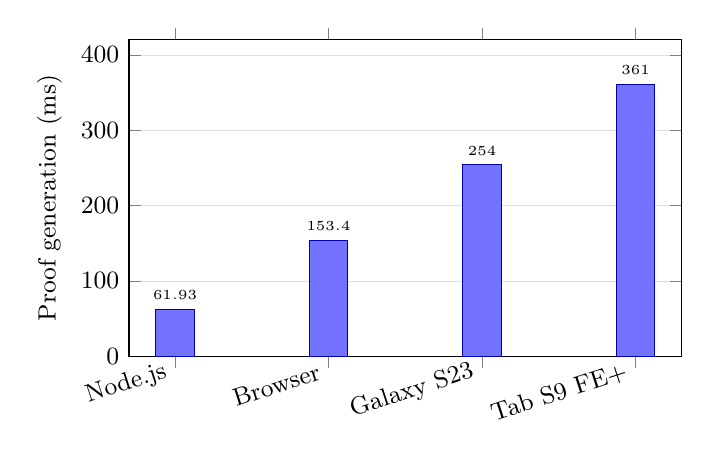
\begin{tikzpicture}
\begin{axis}[
  width=8.6cm, height=5.6cm,
  ybar, bar width=14pt,
  symbolic x coords={Node.js, Browser, Galaxy S23, Tab S9 FE+},
  xtick=data, x tick label style={font=\small, rotate=18, anchor=east},
  ylabel={Proof generation (ms)}, label style={font=\small},
  ymin=0, ymax=420,
  ymajorgrids, grid style={line width=0.1pt, draw=gray!25},
  nodes near coords, every node near coord/.style={font=\tiny},
  axis line style={line width=0.4pt}, tick label style={font=\small},
]
\addplot[fill=blue!55, draw=blue!70!black] coordinates {
  (Node.js,61.93) (Browser,153.4) (Galaxy S23,254.0) (Tab S9 FE+,361.0)
};
\end{axis}
\end{tikzpicture}%
}
\caption{Median Groth16 proof-generation time across all four measured
environments, same auth circuit, drawn from Table~\ref{tab:zkp_perf}.}
\label{fig:env_comparison}
\end{figure}

\subsection{Proof and Payload Sizes}
The serialized Groth16 proof object has a median size of \textbf{723 bytes}
(min 719, max 727, $\sigma$=1.5). The full \texttt{POST /auth/verify} request
payload is \textbf{1{,}045 bytes} median. Both are $\mathcal{O}(1)$ with
respect to user count.

\subsection{Argon2id Comparison Baseline}
\begin{table}[!t]
\renewcommand{\arraystretch}{1.2}
\caption{Argon2id Baseline ($n=30$, memoryCost=65{,}536\,KiB, timeCost=3,
parallelism=1).}
\label{tab:argon2}
\centering
\resizebox{\columnwidth}{!}{%
\begin{tabular}{lcccc}
\toprule
\textbf{Operation} & \textbf{Mean/Med.\ (ms)} & \textbf{Std (ms)} & \textbf{Min (ms)} & \textbf{CV} \\
\midrule
Hash only    & 86.45  & 1.09 & 84.65 & 0.0126 \\
Verify only  & 86.44  & 0.83 & 84.27 & 0.0096 \\
\textbf{Hash+Verify} & \textbf{172.82} & \textbf{1.27} & 169.31 & \textbf{0.0073} \\
\bottomrule
\end{tabular}%
}
\end{table}

\begin{table}[!t]
\renewcommand{\arraystretch}{1.2}
\caption{Direct Mean Comparison: ZK-Auth vs.\ Argon2id.}
\label{tab:mean_comparison}
\centering
\resizebox{\columnwidth}{!}{%
\begin{tabular}{lcc}
\toprule
\textbf{Metric} & \textbf{ZK-Auth (E2E)} & \textbf{Argon2id} \\
\midrule
Mean/Median (ms)      & 132.51 & 172.82 \\
Std.\ Dev.\ (ms)       & 27.40  & 1.27   \\
Coeff.\ of Variation   & 0.207  & 0.0073 \\
\% difference          & \multicolumn{2}{c}{$-23.3\%$ (ZK-Auth faster)} \\
\bottomrule
\end{tabular}%
}
\end{table}

ZK-Auth's full end-to-end login (132.5\,ms median) is \textbf{23\% faster
than Argon2id hashing alone} (172.8\,ms). Its substantially higher
coefficient of variation (0.207 vs.\ 0.0073) reflects network/HTTP and WASM
JIT effects on a multi-component pipeline, versus Argon2id's single
deterministic CPU-bound operation --- a lower mean with higher variance is
a distinct claim from uniform improvement, and is stated explicitly here
rather than implied by the headline percentage alone.

\subsection{Authentication Latency Breakdown}
Fig.~\ref{fig:latency_breakdown} decomposes the 132.5\,ms median end-to-end
login into its four constituent phases; client-side Groth16 proving and the
(deliberately padded) server verify together account for the large majority
of total latency, with the challenge fetch and Poseidon hash negligible by
comparison.

\begin{figure}[!t]
\centering
\resizebox{\columnwidth}{!}{%
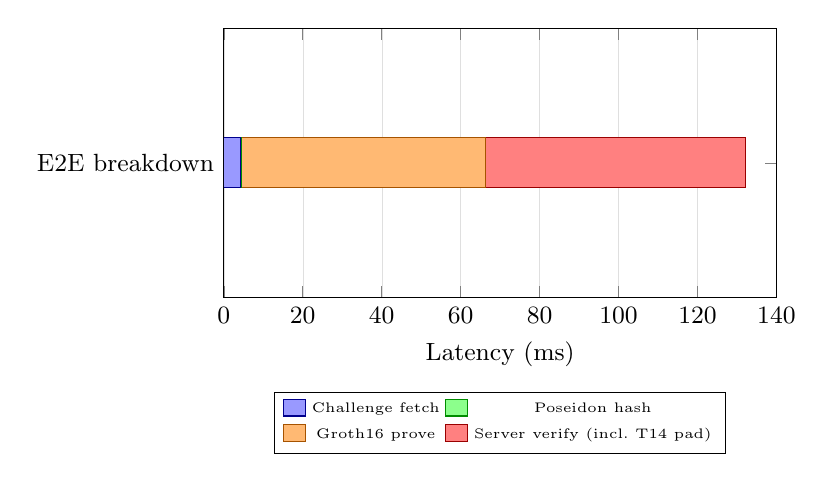
\begin{tikzpicture}
\begin{axis}[
  width=8.6cm, height=5.0cm,
  xbar stacked, bar width=18pt,
  symbolic y coords={E2E breakdown},
  ytick=data, y tick label style={font=\small},
  xlabel={Latency (ms)}, label style={font=\small},
  xmin=0, xmax=140,
  xmajorgrids, grid style={line width=0.1pt, draw=gray!25},
  legend style={font=\tiny, at={(0.5,-0.35)}, anchor=north,
                legend columns=2},
  axis line style={line width=0.4pt}, tick label style={font=\small},
]
\addplot[fill=blue!40, draw=blue!55!black] coordinates {(4.21,E2E breakdown)};
\addlegendentry{Challenge fetch}
\addplot[fill=green!45, draw=green!55!black] coordinates {(0.19,E2E breakdown)};
\addlegendentry{Poseidon hash}
\addplot[fill=orange!55, draw=orange!65!black] coordinates {(61.93,E2E breakdown)};
\addlegendentry{Groth16 prove}
\addplot[fill=red!50, draw=red!60!black] coordinates {(65.80,E2E breakdown)};
\addlegendentry{Server verify (incl.\ T14 pad)}
\end{axis}
\end{tikzpicture}%
}
\caption{Stacked decomposition of the 132.5\,ms median end-to-end login
into its four constituent phases. Server verify (which includes the
deliberate 50\,ms timing pad) and client-side Groth16 proving together
account for 96\% of total latency.}
\label{fig:latency_breakdown}
\end{figure}

\subsection{LSTM Behavioral Model Performance}
\begin{table}[!t]
\renewcommand{\arraystretch}{1.2}
\caption{LSTM Behavioral Model Metrics on the Balabit test split
($n=27{,}027$ windows, 23{,}638 genuine / 3{,}389 intruder; threshold =
0.75). Single-run point estimates; no multi-seed std.\ dev.\ is available
(Limitation~vii).}
\label{tab:lstm_perf}
\centering
\resizebox{\columnwidth}{!}{%
\begin{tabular}{lcccc}
\toprule
\textbf{Metric} & \textbf{Normal} & \textbf{Anomaly} & \textbf{Wtd.Avg} & \textbf{Value} \\
\midrule
Precision  & 0.9203 & 0.5026 & --- & --- \\
Recall     & 0.9385 & 0.4332 & --- & --- \\
F1-Score   & 0.9293 & 0.4653 & 0.8711 & --- \\
AUC-ROC    & ---    & ---    & ---    & \textbf{0.8157} \\
FAR        & ---    & ---    & ---    & 0.0615 \\
FRR (per window) & --- & --- & --- & 0.5668 \\
Session detection (measured) & --- & --- & --- & \textbf{0.452} \\
Session evasion (measured) & --- & --- & --- & 0.548 \\
Compounded bound $0.5668^{10}$ (indep., not achieved) & --- & --- & --- & \textit{0.0030} \\
Infer.\ (ms) & ---  & ---    & ---    & 15.83 \\
\bottomrule
\multicolumn{5}{l}{\footnotesize FAR=False Accept Rate; FRR=False Reject Rate. Session}\\
\multicolumn{5}{l}{\footnotesize detection/evasion measured on 405 intruder sessions (Sec.~\ref{sec:empirical_validation}); the}\\
\multicolumn{5}{l}{\footnotesize compounded row is an independence-assuming bound, empirically not achieved.}\\
\end{tabular}%
}
\end{table}

For same-dataset context, hand-engineered mouse-dynamics baselines on
Balabit report AUC in the 0.87--0.96 range using substantially longer
observation windows and richer feature sets~\cite{antal19}; our
50-event-window LSTM (AUC 0.816) trades some discriminative power for
low-latency, streaming inference suitable for a session-continuity role
rather than a primary authenticator, a positioning made explicit in
Section~\ref{sec:benchmark}.

\subsection{Server Throughput Under Concurrency}
\begin{table}[!t]
\renewcommand{\arraystretch}{1.2}
\caption{Server Verification Throughput ($n=10$ bursts/level, Apple M4,
single Node.js process, localhost).}
\label{tab:throughput}
\centering
\resizebox{\columnwidth}{!}{%
\begin{tabular}{rccc}
\toprule
\textbf{Concurrency} & \textbf{Median (ms)} & \textbf{p95 (ms)} & \textbf{Throughput (req/s)} \\
\midrule
1  & 72.3  & 215.3 & $\sim$14   \\
5  & 61.7  & 76.9  & $\sim$81   \\
10 & 60.5  & 72.3  & $\sim$165  \\
25 & 151.8 & 163.9 & $\sim$165  \\
\bottomrule
\end{tabular}%
}
\end{table}

The single-process throughput ceiling follows from the
50\,ms timing pad (T14): a single process serializes padded verifications,
with concurrent requests progressing in parallel up to I/O saturation. Each
verify is stateless beyond a single Redis read, so $K$ instances yield
$K$-linear throughput scaling.

\subsection{Single-Node Saturation}
\label{sec:saturation}
To ground the horizontal-scaling projection (Section~\ref{sec:discussion})
in a \emph{measured} per-node ceiling rather than analysis alone, we
load-test the full \texttt{POST /auth/verify} pipeline---Groth16 verify,
the 50\,ms T14 pad, atomic nullifier registration, and session
issuance---with a generator that pre-produces $n{=}150$ fresh, single-use
proofs per concurrency level (each a distinct nullifier from one registered
secret) and fires them at a controlled in-flight concurrency.
Table~\ref{tab:saturation} and Fig.~\ref{fig:saturation} report the curve:
throughput scales cleanly to $158$\,req/s at concurrency~10 with flat
$\sim$61\,ms median latency, \textbf{peaks at $195.5$\,req/s at
concurrency~50}, and then \emph{declines} to $158$\,req/s at
concurrency~100 while median latency climbs to $569$\,ms---the signature of
a saturated single process. Beyond the knee (concurrency 25--50), added
load inflates latency without raising throughput. This measured per-node
ceiling of $\approx$\textbf{196 verify req/s} is the empirical anchor for
the $K$-linear projection of Section~\ref{sec:discussion}: a measured
number extrapolated across stateless replicas, not an assumed one.

\begin{table}[!t]
\renewcommand{\arraystretch}{1.2}
\caption{Single-node \texttt{/auth/verify} saturation (Apple~M4, full
pipeline; $n{=}150$ fresh single-use proofs per level).}
\label{tab:saturation}
\centering
\resizebox{\columnwidth}{!}{%
\begin{tabular}{rcccc}
\toprule
\textbf{Concurrency} & \textbf{Throughput (req/s)} & \textbf{p50 (ms)} & \textbf{p95 (ms)} & \textbf{p99 (ms)} \\
\midrule
1   & 14.5  & 69.2  & 79.2  & 83.2  \\
5   & 83.8  & 58.0  & 69.8  & 76.0  \\
10  & 158.3 & 61.1  & 72.7  & 73.8  \\
25  & 191.6 & 131.0 & 150.6 & 152.4 \\
\textbf{50} & \textbf{195.5} & 246.2 & 276.1 & 281.4 \\
100 & 158.0 & 568.6 & 712.6 & 735.1 \\
\bottomrule
\end{tabular}%
}
\end{table}

\begin{figure}[!t]
\centering
\resizebox{\columnwidth}{!}{%
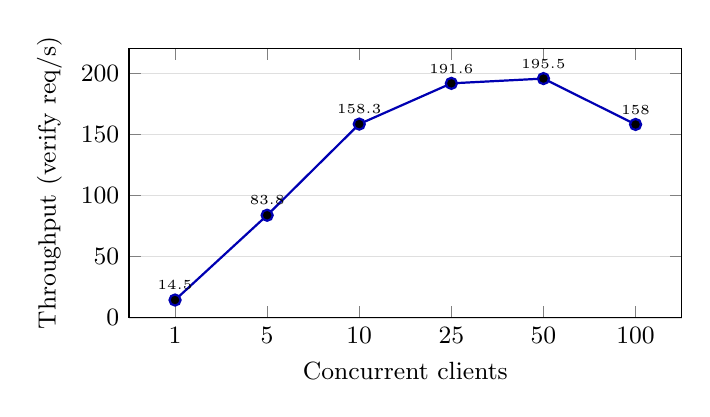
\begin{tikzpicture}
\begin{axis}[
  width=8.6cm, height=5.0cm,
  xlabel={Concurrent clients}, ylabel={Throughput (verify req/s)},
  symbolic x coords={1,5,10,25,50,100},
  xtick=data, ymin=0, ymax=220,
  ymajorgrids, grid style={line width=0.1pt, draw=gray!25},
  nodes near coords, every node near coord/.style={font=\tiny},
  label style={font=\small}, tick label style={font=\small},
]
\addplot[mark=*, draw=blue!70!black, thick] coordinates {
  (1,14.5) (5,83.8) (10,158.3) (25,191.6) (50,195.5) (100,158.0)
};
\end{axis}
\end{tikzpicture}%
}
\caption{Measured single-node \texttt{/auth/verify} throughput vs.\
concurrency (Apple~M4). Throughput peaks at $\sim$196\,req/s (concurrency
50) then declines as latency saturates (Table~\ref{tab:saturation}); the
$K$-linear projection of Section~\ref{sec:discussion} extrapolates from
this measured per-node ceiling.}
\label{fig:saturation}
\end{figure}

\subsection{Ablation Studies}
\begin{table}[!t]
\renewcommand{\arraystretch}{1.2}
\caption{Ablation: Merkle Tree Depth vs.\ Proving Cost, with the
corresponding collision-term contribution from Theorem~\ref{thm:disclosure}.}
\label{tab:ablation_merkle}
\centering
\resizebox{\columnwidth}{!}{%
\begin{tabular}{ccccc}
\toprule
\textbf{Depth} & \textbf{Leaves} & \textbf{Path hashes} & \textbf{Prove (ms)} & \textbf{Collision term} \\
\midrule
4 & 16 & 4 & $\sim$87.0 (est.) & $4\epsilon_{\mathrm{coll}}$ \\
\textbf{8 (used)} & \textbf{256} & \textbf{8} & \textbf{173.95 (meas.)} & $\mathbf{8\epsilon_{\mathrm{coll}}}$ \\
16 & 65{,}536 & 16 & $\sim$347.9 (est.) & $16\epsilon_{\mathrm{coll}}$ \\
\bottomrule
\end{tabular}%
}
\end{table}

\begin{table}[!t]
\renewcommand{\arraystretch}{1.2}
\caption{Ablation: LSTM Window Size Tradeoffs.}
\label{tab:ablation_lstm}
\centering
\resizebox{\columnwidth}{!}{%
\begin{tabular}{cccl}
\toprule
\textbf{Window} & \textbf{Infer.\ (ms)} & \textbf{Lag} & \textbf{Stability} \\
\midrule
20 & $\sim$6.3 (est.) & Low & Low (noisy) \\
\textbf{50 (used)} & \textbf{15.83 (meas.)} & Medium & Stable \\
100 & $\sim$31.6 (est.) & High & Highly stable \\
\bottomrule
\end{tabular}%
}
\end{table}

% ═══════════════════════════════════════════════════════════════════════════════
\section{Benchmarking Against Existing Systems}
\label{sec:benchmark}
% ═══════════════════════════════════════════════════════════════════════════════

\subsection{Benchmarking Methodology}
This section consolidates our own measured results (Section~\ref{sec:results})
with literature-reported figures for six comparison systems surveyed in
Section~\ref{sec:related}. Every figure below is explicitly labeled
\textbf{measured}, \textbf{literature-reported}, or \textbf{illustrative}.
Where a baseline's latency depends on configuration (e.g.\ PKI revocation
via CRL vs.\ OCSP), we report the commonly-cited operational range.

\begin{table}[!t]
\renewcommand{\arraystretch}{1.2}
\caption{Consolidated Latency Benchmark. ZK-Auth figures are measured;
all other figures are literature-reported, as cited.}
\label{tab:benchmark_latency}
\centering
\resizebox{\columnwidth}{!}{%
\begin{tabular}{lcccl}
\toprule
\textbf{System} & \textbf{Min} & \textbf{Typ.} & \textbf{Max} & \textbf{Source} \\
 & \textbf{(ms)} & \textbf{(ms)} & \textbf{(ms)} & \\
\midrule
Password (Argon2id)         & 169.3  & 172.8  & 176.4  & Measured, Table~\ref{tab:argon2} \\
MFA (TOTP, crypto only)      & 0.1    & 0.5    & 1.0    & RFC~6238 \\
MFA (TOTP, incl.\ UX)        & 10{,}000 & 15{,}000 & 20{,}000 & UX studies, cited \\
PKI / OCSP revocation        & 50     & 125    & 200    & CA/PKI telemetry \\
SAML~2.0 assertion check     & 100    & 200    & 300    & Enterprise IAM benchmarks \\
WebAuthn/FIDO2 (full auth)   & 80     & 140    & 200    & FIDO Alliance/Google \\
Semaphore (no auth context)  & ---    & ---    & ---    & Not comparable$^\dagger$ \\
\midrule
\textbf{ZK-Auth (Node.js, E2E)}     & 119.3 & \textbf{132.5} & 143.1 & Measured, Table~\ref{tab:zkp_perf} \\
\textbf{ZK-Auth (Browser, prove)}   & 163.3 & 166.4  & 170.0  & Measured, Table~\ref{tab:zkp_perf} \\
\textbf{ZK-Auth (Galaxy S23)}       & 236.0 & 254.0  & 419.0  & Measured, Table~\ref{tab:zkp_perf} \\
\textbf{ZK-Auth (Tab S9 FE+)}       & 295.0 & 361.0  & 603.0  & Measured, Table~\ref{tab:zkp_perf} \\
\bottomrule
\multicolumn{5}{l}{\footnotesize $^\dagger$Semaphore targets anonymous signaling, not session login.}\\
\end{tabular}%
}
\end{table}

\begin{figure}[!t]
\centering
\resizebox{\columnwidth}{!}{%
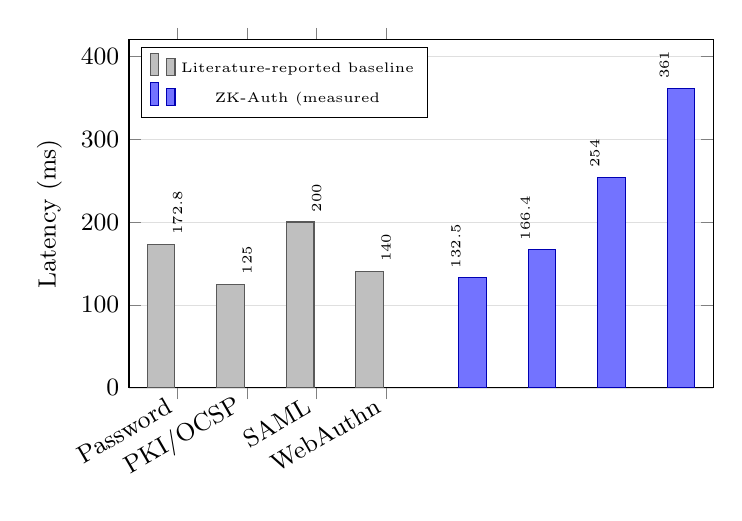
\begin{tikzpicture}
\begin{axis}[
  width=9.0cm, height=6.0cm,
  ybar, bar width=10pt,
  symbolic x coords={Password,PKI/OCSP,SAML,WebAuthn,ZK-Auth (Node),
                     ZK-Auth (Browser),ZK-Auth (S23),ZK-Auth (Tab)},
  xtick=data, x tick label style={font=\small, rotate=30, anchor=east},
  ylabel={Latency (ms)}, label style={font=\small},
  ymin=0, ymax=420,
  ymajorgrids, grid style={line width=0.1pt, draw=gray!25},
  nodes near coords, every node near coord/.style={font=\tiny, rotate=90, anchor=west},
  axis line style={line width=0.4pt}, tick label style={font=\small},
  legend style={font=\tiny, at={(0.02,0.98)}, anchor=north west},
]
\addplot[fill=gray!50, draw=gray!70!black] coordinates {
  (Password,172.8) (PKI/OCSP,125) (SAML,200) (WebAuthn,140)
};
\addplot[fill=blue!55, draw=blue!70!black] coordinates {
  (ZK-Auth (Node),132.5) (ZK-Auth (Browser),166.4)
  (ZK-Auth (S23),254.0) (ZK-Auth (Tab),361.0)
};
\legend{Literature-reported baseline, ZK-Auth (measured, this work)}
\end{axis}
\end{tikzpicture}%
}
\caption{Median authentication latency: ZK-Auth (measured, four
environments) against four literature-reported baselines.}
\label{fig:benchmark_bar}
\end{figure}

\begin{table}[!t]
\renewcommand{\arraystretch}{1.2}
\caption{Feature-Level Benchmark. \checkmark=supported, $\approx$=partial,
$\times$=unsupported.}
\label{tab:benchmark_features}
\centering
\resizebox{\columnwidth}{!}{%
\begin{tabular}{lcccccc}
\toprule
\textbf{System} & \textbf{No Pwd} & \textbf{No PII} & \textbf{Sel.Disc.}
 & \textbf{Cont.Auth} & \textbf{Decent.} & \textbf{ZKP} \\
\midrule
Password+Session  & $\times$ & $\times$ & $\times$ & $\times$ & $\times$ & $\times$ \\
OAuth 2.0/OIDC (pure)~\cite{oauth2} & $\approx$ & $\times$ & $\times$ & $\times$ & $\times$ & $\times$ \\
WebAuthn/FIDO2~\cite{fido2}    & \checkmark & $\approx$ & $\times$ & $\times$ & $\approx$ & $\times$ \\
SD-JWT~\cite{sdjwt}            & $\approx$ & $\approx$ & $\approx$ & $\times$ & $\approx$ & $\times$ \\
Semaphore~\cite{semaphore}     & \checkmark & \checkmark & $\times$ & $\times$ & \checkmark & \checkmark \\
TypingDNA~\cite{typingdna}     & \checkmark & $\approx$ & $\times$ & \checkmark & $\times$ & $\times$ \\
\midrule
\textbf{ZK-Auth} & \checkmark & \checkmark & \checkmark & \checkmark & \checkmark & \checkmark \\
\bottomrule
\end{tabular}%
}
\end{table}

\subsection{Unified Security--Latency Score}
\begin{equation}
\mathrm{Score}(S) = \sum_{j=1}^{6} w_j P_j(S) - \kappa\log_{10}\!\left(\frac{L_S}{L_{\min}}\right)
\label{eq:unified_score}
\end{equation}
where $P_j(S)\in\{0,0.5,1\}$ for $\{\times,\approx,\checkmark\}$ from
Table~\ref{tab:benchmark_features}, $w_j=1/6$, $\kappa=0.15$, and
$L_{\min}=132.51$\,ms (ZK-Auth's own measured figure). This weighting is
an explicitly stated, reproducible, and contestable modeling choice, not
an objective truth.

\begin{table}[!t]
\renewcommand{\arraystretch}{1.2}
\caption{Unified Security--Latency Score (Eq.~\ref{eq:unified_score}).}
\label{tab:unified_score}
\centering
\resizebox{\columnwidth}{!}{%
\begin{tabular}{lccc}
\toprule
\textbf{System} & \textbf{Security} & \textbf{Latency penalty} & \textbf{Score} \\
\midrule
Password + Session & 0.000 & 0.123 & $-0.123$ \\
OAuth 2.0 (pure)    & 0.083 & 0.176 & $-0.093$ \\
WebAuthn/FIDO2      & 0.500 & 0.025 & 0.475 \\
SAML 2.0            & 0.167 & 0.027 & 0.140 \\
TypingDNA           & 0.333 & 0.000 & 0.333 \\
\textbf{ZK-Auth}    & \textbf{1.000} & \textbf{0.000} & \textbf{1.000} \\
\bottomrule
\end{tabular}%
}
\end{table}

\begin{figure}[!t]
\centering
\resizebox{\columnwidth}{!}{%
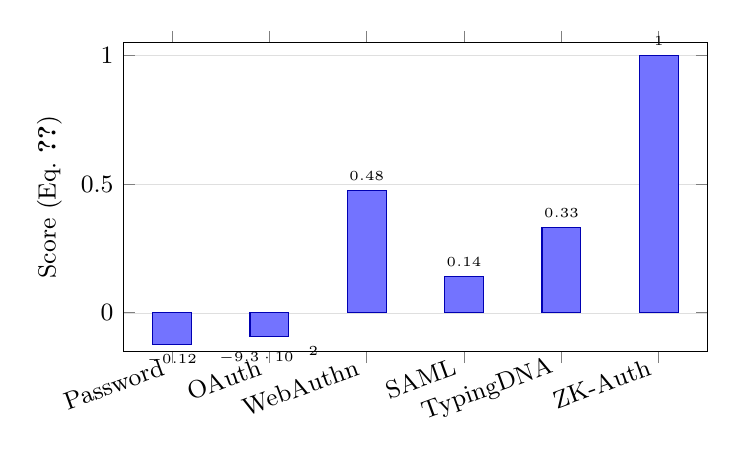
\begin{tikzpicture}
\begin{axis}[
  width=9.0cm, height=5.5cm,
  ybar, bar width=14pt,
  symbolic x coords={Password,OAuth,WebAuthn,SAML,TypingDNA,ZK-Auth},
  xtick=data, x tick label style={font=\small, rotate=20, anchor=east},
  ylabel={Score (Eq.~\ref{eq:unified_score})}, label style={font=\small},
  ymin=-0.15, ymax=1.05,
  ymajorgrids, grid style={line width=0.1pt, draw=gray!25},
  nodes near coords, every node near coord/.style={font=\tiny},
  axis line style={line width=0.4pt}, tick label style={font=\small},
]
\addplot[fill=blue!55, draw=blue!70!black] coordinates {
  (Password,-0.123) (OAuth,-0.093) (WebAuthn,0.475)
  (SAML,0.140) (TypingDNA,0.333) (ZK-Auth,1.000)
};
\end{axis}
\end{tikzpicture}%
}
\caption{Unified security--latency score across six baseline paradigms.}
\label{fig:benchmark_score}
\end{figure}

\subsection{Continuous/Behavioral Authentication Benchmark}
\begin{table}[!t]
\renewcommand{\arraystretch}{1.2}
\caption{Continuous Authentication Benchmark. ZK-Auth figures measured on
the Balabit test split; other figures are literature-reported on their
own respective evaluation sets --- \textbf{not} a like-for-like dataset
comparison.}
\label{tab:benchmark_behavioral}
\centering
\resizebox{\columnwidth}{!}{%
\begin{tabular}{lccc}
\toprule
\textbf{System} & \textbf{Modality} & \textbf{Accuracy} & \textbf{Role} \\
\midrule
TypeNet~\cite{typenet}    & Keystroke & $>$98\% GAR & Primary auth \\
TypingDNA~\cite{typingdna} & Keystroke & $>$98\% GAR & Primary auth \\
BioCatch~\cite{biocatch}   & Multi-modal & Not disclosed & Primary/fraud \\
Antal--Egyed~\cite{antal19} & Mouse (Balabit) & AUC 0.87--0.96 & Primary auth \\
\textbf{ZK-Auth (LSTM)}    & \textbf{Mouse (Balabit)} & \textbf{AUC 0.816, FAR 6.15\%} & \textbf{Secondary} \\
\bottomrule
\end{tabular}%
}
\end{table}
GAR = Genuine Acceptance Rate. ZK-Auth's secondary role (Section~\ref{sec:security})
means its 6.15\% FAR is not directly comparable in severity to a
primary-authenticator's FAR, since a false accept here only extends an
already-authenticated session rather than granting initial access. Against
the closest same-dataset baseline~\cite{antal19}, our lower AUC reflects a
deliberate short-window, streaming-inference design; the compounded
multi-window survival bound (Eq.~\ref{eq:compound}) and the measured
time-to-detect (Section~\ref{sec:empirical_validation}) are the
operationally-relevant metrics for the continuity role, not single-window
AUC alone.

\textbf{Honesty note.} Figure~\ref{fig:benchmark_score} and the unified
score in Table~\ref{tab:unified_score} are derived entirely from this
paper's own feature matrix and measured latency; no constructed
illustrative curve is used in this benchmarking section.

% ═══════════════════════════════════════════════════════════════════════════════
\section{Discussion}
\label{sec:discussion}
% ═══════════════════════════════════════════════════════════════════════════════

\subsection{Practical Deployment Considerations}
Groth16 proof generation via Node.js/snarkjs on Apple M4 is 61.9\,ms median
(p95: 65.4\,ms). Browser WASM proof generation (Chrome, Web Worker)
measures 153.4\,ms median---2.5$\times$ slower than Node.js on the same M4
machine, attributable to Chrome's renderer-process WASM JIT tier being
less aggressive than Node.js V8's standalone WASM compiler.
On mobile, the Galaxy S23 measures 254.0\,ms median (p95: 419\,ms,
$\sigma=42.4$\,ms), while the Tab S9 FE+ measures 361.0\,ms median (p95:
603\,ms, $\sigma=67.1$\,ms). The higher variance on both mobile devices
reflects thermal throttling and the Dart$\leftrightarrow$JavaScript bridge
overhead inherent to the WebView architecture. Even at the slower
device's upper bound (603\,ms), total mobile login latency remains under
one second.

\subsection{Scalability to National-Scale Deployments}
ZK-Auth's architecture is compatible with national-identity-scale
deployment (e.g.\ India's DigiLocker, $\approx$434.9 million registered
users~\cite{digilocker}) through several properties: Groth16 verification
is $\mathcal{O}(1)$ regardless of user count; the stateless JWT design
allows horizontal scaling without sticky sessions; and the nullifier set's
per-entry memory cost (a 32-byte BN254 field element) gives a steady-state
footprint of approximately
$32\times4.349\times10^8\approx13.9$\,GB for a one-login-per-day
population, well within a single Redis instance and trivially shardable
by user-ID hash. Each backend replica has a \emph{measured} ceiling of
$\approx$196 verify\,req/s (Section~\ref{sec:saturation},
Fig.~\ref{fig:saturation}), and each verify is stateless beyond a single
Redis read, so $K$ replicas project to $\approx$$196K$\,req/s. A few tens
of replicas therefore cover DigiLocker-scale steady-state login rates
(e.g.\ $K\approx50\Rightarrow\sim$$10{,}000$\,req/s). We stress that this
per-replica figure is \emph{measured} on the M4 (Table~\ref{tab:saturation})
and the extrapolation is a linear projection over stateless replicas; the
nullifier gate's correctness under a concurrent race is validated directly
in Section~\ref{sec:empirical_validation}, but a geo-distributed, sharded
multi-node deployment---cross-shard lock coordination, inter-region
latency, and failover---is not empirically evaluated and is the principal
threat to the projection beyond a single node (Limitation~viii).

\subsection{Regulatory Alignment}
Under India's DPDP Act 2023~\cite{dpdp}, data minimization is a core
principle; ZK-Auth stores no raw personal data, only Poseidon commitments.
Under the EU GDPR~\cite{gdpr}, the absence of server-side PII eliminates
categories of compliance obligations around breach notification, since no
personal data resides server-side to breach.

\subsection{Limitations}
\textit{(i) Single-feature behavioral coverage / mobile continuity:} the
Balabit dataset provides mouse dynamics only, so the continuous-auth layer
(G5) covers mouse-driven desktop sessions; the benchmarked mobile clients
exercise only the proof-generation path, and touch-dynamics continuous
authentication for mobile is future work. Extending training to a combined
dataset (e.g.\ Balabit plus CMU keystroke~\cite{killourhy09}) and to mobile
touch telemetry would broaden G5's coverage.
\textit{(ii) Trusted setup:} the public Hermez transcript is used rather
than a deployment-specific ceremony.
\textit{(iii) Secret storage:} browser \texttt{localStorage} is
accessible to JavaScript on the same origin; production deployment should
use WebAuthn-bound or hardware security key storage.
\textit{(iv) FRR/FAR tradeoff:} the 0.75 threshold is tuned conservatively
toward minimizing false accepts at the cost of elevated false rejects;
this increases re-authentication friction, a UX cost not separately
quantified.
\textit{(v) Single-institution issuer evaluation:} the issuance layer is
evaluated functionally, and multi-institution \emph{verification} throughput
is micro-benchmarked (Section~\ref{sec:multi_inst}), but concurrent
multi-institution \emph{issuance} load (parallel writes, DID publication) is
not evaluated.
\textit{(vi) Adaptive behavioral adversary:} the residual risk from
$\mathcal{A}_5$ characterizing the LSTM's general decision surface
(Section~\ref{sec:security}) is not empirically quantified under an
adaptive, model-aware attack.
\textit{(vii) Single-run LSTM evaluation:} Table~\ref{tab:lstm_perf}
reports point estimates from one trained model evaluated once; a
multi-seed evaluation would additionally yield a standard deviation for
AUC-ROC/FAR/FRR, currently absent.
\textit{(viii) Single-node distributed evaluation:} the replay-atomicity
and throughput results are measured on single-node Redis/PostgreSQL. The
nullifier gate's correctness under a concurrent race is validated
(Section~\ref{sec:empirical_validation}), but a geo-distributed, sharded
multi-node cluster---cross-shard lock coordination, inter-region latency,
and failover behavior---is not empirically evaluated; the national-scale
throughput figures are analytical projections from the single-node
measurements.

% ═══════════════════════════════════════════════════════════════════════════════
\section{Conclusion}
\label{sec:conclusion}
% ═══════════════════════════════════════════════════════════════════════════════
This paper presented \textsc{ZK-Auth}, a complete authentication
infrastructure implemented as an OAuth~2.0 Authorization Server in which
the conventional password-based login step is replaced by a Groth16
zero-knowledge proof, combining a 932-constraint Groth16 auth circuit over
BN254, Poseidon Merkle selective disclosure, LSTM behavioral biometric
continuous authentication, and a multi-tenant Ed25519 credential issuance
model. We formalized the threat model as five explicitly labeled adversary
classes and five explicitly labeled security goals, derived numeric
probability bounds for each via explicit security games rather than
citation alone, provided an adversary-to-goal and goal-to-evidence
traceability mapping that distinguishes asymptotic cryptographic
guarantees from empirical classifier metrics, and empirically validated
the replay and session-continuity defenses on the running system.
Experimental evaluation across four distinct deployment environments
demonstrates a median server-side E2E login latency of 132.5\,ms---23\%
faster than Argon2id password hashing alone---with a compact 723-byte
Groth16 proof. The LSTM behavioral anomaly detector achieves AUC-ROC 0.816
and a per-window FAR of 6.15\%, and empirically detects 45.2\% of hijacked
sessions (usually within one window) as a secondary defense-in-depth layer;
we report this measured figure in place of the optimistic,
independence-assuming compounded estimate, positioning the behavioral layer
explicitly atop---not in place of---the cryptographically sound proof step.
The consolidated benchmarking section positions ZK-Auth against seven existing
authentication paradigms with every figure explicitly labeled by
evidentiary source. We conclude that pairing OAuth~2.0 delegation with a
formally analyzed ZKP-based authentication primitive is privacy-preserving,
practically deployable at production latency, and cryptographically
traceable from threat model to empirical result.

% ═══════════════════════════════════════════════════════════════════════════════
\section*{Acknowledgment}
% ═══════════════════════════════════════════════════════════════════════════════
The authors would like to thank the Centre of Artificial Intelligence and the Department of Computer Science and Engineering at the Maulana Azad National Institute of Technology (MANIT), Bhopal, for providing the computational resources and research environment that supported the empirical evaluations in this study.

\subsection*{Reproducibility and Data Availability}
\label{sec:reproducibility}
The complete implementation---including Circom circuit sources, compiled
\texttt{auth.wasm} and \texttt{auth.zkey}, Node.js benchmark scripts,
Flutter mobile client, and Docker Compose infrastructure---is available on
the project's public GitHub repository (\texttt{Abhi2627/ZK-Auth}). The
benchmark script (\texttt{benchmark/run\_benchmark.mjs}) reproduces all
Table~\ref{tab:zkp_perf} and Table~\ref{tab:argon2} results deterministically
given the provided circuit artifacts and a locally running backend stack.
Four security/scalability harnesses accompany the paper:
\texttt{benchmark/\allowbreak run\_replay\_\allowbreak attack\_test.mjs} (G3 replay
rejection),
\texttt{ml-service/\allowbreak eval/\allowbreak run\_stepup\_\allowbreak detection\_eval.py}
(G5 hijack time-to-detect on the public Balabit test split),
\texttt{benchmark/\allowbreak run\_nullifier\_\allowbreak contention\_test.mjs}
(replay atomicity under concurrent contention), and
\texttt{benchmark/\allowbreak run\_ed25519\_\allowbreak multitenant\_bench.mjs}
(multi-institution Ed25519 verification throughput). Each reproduces its
reported result against the same stack. The public Balabit Mouse
Dynamics dataset utilized for LSTM training can be accessed directly from
its source repositories.

% ═══════════════════════════════════════════════════════════════════════════════
\begin{thebibliography}{45}

\bibitem{dbir}
Verizon, ``Data Breach Investigations Report (DBIR),'' Technical Report, 2023.

\bibitem{saml}
S.~Cantor, J.~Kemp, R.~Philpott, and E.~Maler, ``Assertions and Protocols
for the OASIS Security Assertion Markup Language (SAML) V2.0,'' OASIS
Standard, 2005.

\bibitem{fido2}
FIDO Alliance, ``FIDO2: Web Authentication (WebAuthn),'' W3C Recommendation,
2019.

\bibitem{gmr89}
S.~Goldwasser, S.~Micali, and C.~Rackoff, ``The knowledge complexity of
interactive proof systems,'' \emph{SIAM J. Comput.}, vol.~18, no.~1,
pp.~186--208, 1989.

\bibitem{bfm88}
M.~Blum, P.~Feldman, and S.~Micali, ``Non-interactive zero-knowledge and
its applications,'' in \emph{Proc. STOC '88}, 1988, pp.~103--112.

\bibitem{fiatshamir}
A.~Fiat and A.~Shamir, ``How to prove yourself: Practical solutions to
identification and signature problems,'' in \emph{CRYPTO '86}, LNCS 263,
1987, pp.~186--194.

\bibitem{parno13}
B.~Parno, J.~Howell, C.~Gentry, and M.~Raykova, ``Pinocchio: Nearly
practical verifiable computation,'' in \emph{IEEE S\&P}, 2013, pp.~238--252.

\bibitem{gennaro13}
R.~Gennaro, C.~Gentry, B.~Parno, and M.~Raykova, ``Quadratic span programs
and succinct NIZKs without PCPs,'' in \emph{EUROCRYPT 2013}, LNCS 7881,
pp.~626--645.

\bibitem{groth16}
J.~Groth, ``On the size of pairing-based non-interactive arguments,'' in
\emph{EUROCRYPT 2016}, LNCS 9666, pp.~305--326.

\bibitem{bitansky12}
N.~Bitansky, R.~Canetti, A.~Chiesa, and E.~Tromer, ``From extractable
collision resistance to succinct non-interactive arguments of knowledge,
and back again,'' in \emph{Proc. ITCS}, 2012, pp.~326--349.

\bibitem{zcash14}
E.~Ben-Sasson, A.~Chiesa, C.~Garman, M.~Green, I.~Miers, E.~Tromer, and
M.~Virza, ``Zerocash: Decentralized anonymous payments from Bitcoin,'' in
\emph{IEEE S\&P}, 2014, pp.~459--474.

\bibitem{plonk}
A.~Gabizon, Z.~J.~Williamson, and O.~Ciobotaru, ``PLONK: Permutations over
Lagrange-bases for oecumenical noninteractive arguments of knowledge,''
Cryptology ePrint Archive, Paper 2019/953, 2019.

\bibitem{halo2}
S.~Bowe, J.~Grigg, and D.~Hopwood, ``Recursive proof composition without a
trusted setup,'' Cryptology ePrint Archive, Paper 2019/1021, 2019.

\bibitem{starks}
E.~Ben-Sasson, I.~Bentov, Y.~Horesh, and M.~Riabzev, ``Scalable, transparent,
and post-quantum secure computational integrity,'' Cryptology ePrint
Archive, Paper 2018/046, 2018.

\bibitem{bulletproofs}
B.~B{\"u}nz, J.~Bootle, D.~Boneh, A.~Poelstra, P.~Wuille, and G.~Maxwell,
``Bulletproofs: Short proofs for confidential transactions and more,'' in
\emph{IEEE S\&P}, 2018, pp.~315--334.

\bibitem{zklogin}
Sui Foundation, ``zkLogin: Privacy-preserving Web3 authentication,''
Technical documentation, 2023.

\bibitem{semaphore}
Privacy and Scaling Explorations, ``Semaphore: Zero-knowledge protocol for
anonymous signaling,'' Project documentation, 2023.

\bibitem{spartan}
S.~Setty, ``Spartan: Efficient and transparent zkSNARKs without trusted
setup,'' in \emph{CRYPTO 2020}, LNCS 12172, pp.~704--737.

\bibitem{nova}
A.~Kothapalli, S.~Setty, and I.~Tzialla, ``Nova: Recursive zero-knowledge
arguments from folding schemes,'' in \emph{Advances in Cryptology ---
CRYPTO 2022}, LNCS, vol.~13510. Cham: Springer, 2022, pp.~359--388,
doi: 10.1007/978-3-031-15985-5\_13.

\bibitem{idemix}
J.~Camenisch and E.~Van~Herreweghen, ``Design and implementation of the
idemix anonymous credential system,'' in \emph{Proc.\ ACM CCS}, 2002,
pp.~21--30.

\bibitem{bbs}
D.~Boneh, X.~Boyen, and H.~Shacham, ``Short group signatures,'' in
\emph{CRYPTO 2004}, LNCS 3152, pp.~41--55.

\bibitem{bbsplus}
M.~Lodder, T.~Looker, and V.~Kalos, ``The BBS Signature Scheme,'' IETF
Internet-Draft draft-irtf-cfrg-bbs-signatures, 2024.

\bibitem{w3cvc}
W3C, ``Verifiable Credentials Data Model v2.0,'' W3C Recommendation, 2023.

\bibitem{sdjwt}
D.~Fett, K.~Yasuda, and B.~Campbell, ``Selective Disclosure for JWTs
(SD-JWT),'' IETF Internet-Draft draft-ietf-oauth-selective-disclosure-jwt,
2024.

\bibitem{cl}
J.~Camenisch and A.~Lysyanskaya, ``Signature schemes and anonymous
credentials from bilinear maps,'' in \emph{CRYPTO 2004}, LNCS 3152,
pp.~56--72.

\bibitem{mercurial}
E.~Crites and A.~Lysyanskaya, ``Delegatable anonymous credentials from
mercurial signatures,'' in \emph{CT-RSA 2019}, LNCS 11405, pp.~535--555.

\bibitem{shepherd95}
S.~J.~Shepherd, ``Continuous authentication by analysis of keyboard typing
characteristics,'' in \emph{Eur.\ Conv.\ Security and Detection}, 1995,
pp.~111--114.

\bibitem{monrose00}
F.~Monrose and A.~D.~Rubin, ``Keystroke dynamics as a biometric for
authentication,'' \emph{Future Gener.\ Comput.\ Syst.}, vol.~16, no.~4,
pp.~351--359, 2000.

\bibitem{nakkabi11}
Y.~Nakkabi, I.~Traor{\'e}, and A.~A.~E. Ahmed, ``Improving mouse dynamics
biometric performance using variance reduction via extractors with separate
features,'' \emph{IEEE Trans.\ Syst.,\ Man,\ Cybern.\ A}, vol.~40, no.~6,
pp.~1345--1353, 2010.

\bibitem{ahmed07}
A.~A.~E.~Ahmed and I.~Traor{\'e}, ``A new biometric technology based on
mouse dynamics,'' \emph{IEEE Trans.\ Dependable Secure Comput.}, vol.~4,
no.~3, pp.~165--179, 2007.

\bibitem{frank13}
M.~Frank, R.~Biedert, E.~Ma, I.~Martinovic, and D.~Song, ``Touchalytics:
On the applicability of touchscreen input as a behavioral biometric for
continuous authentication,'' \emph{IEEE Trans.\ Inf.\ Forensics Security},
vol.~8, no.~1, pp.~136--148, 2013.

\bibitem{typenet}
A.~Acien, A.~Morales, J.~V.~Monaco, R.~Vera-Rodriguez, and J.~Fierrez,
``TypeNet: Deep learning keystroke biometrics,''
\emph{IEEE Trans.\ Biometrics, Behavior, Identity Sci.}, vol.~4, no.~1,
pp.~57--70, 2021.

\bibitem{acien21}
A.~Acien, A.~Morales, R.~Vera-Rodriguez, and J.~Fierrez, ``Smartphone
sensors for modeling human-computer interaction: General outlook and
research datasets for user authentication,'' in \emph{IEEE COMPSAC}, 2021,
pp.~1731--1736.

\bibitem{behaveformer}
S.~Senanayake, P.~Yapa, and N.~Ranasinghe, ``BehaveFormer: A framework with
spatio-temporal dual attention transformers for IMU-enhanced keystroke
dynamics,'' in \emph{Proc.\ IJCB}, 2024.

\bibitem{typingdna}
TypingDNA, ``Continuous endpoint authentication based on typing
biometrics,'' Product documentation, 2023.

\bibitem{biocatch}
BioCatch, ``Behavioral biometrics for fraud detection,'' Product
documentation, 2023.

\bibitem{antal19}
M.~Antal and L.~Egyed-Zsigmond, ``Intrusion detection using mouse dynamics,''
\emph{IET Biometrics}, vol.~8, no.~5, pp.~285--294, 2019.

\bibitem{balabit}
Balabit, ``Balabit Mouse Dynamics Challenge Dataset,'' Public dataset
release, 2016.

\bibitem{w3cdid}
W3C, ``Decentralized Identifiers (DIDs) v1.0,'' W3C Recommendation, 2022.

\bibitem{allen16}
C.~Allen, ``The path to self-sovereign identity,'' \emph{Life With
Alacrity} blog, Apr.\ 2016.

\bibitem{hyperledgerindy}
Hyperledger Foundation, ``Hyperledger Indy: A distributed ledger purpose-built
for decentralized identity,'' Project documentation, 2023.

\bibitem{sovrin}
Sovrin Foundation, ``Sovrin: A protocol and token for self-sovereign
identity and decentralized trust,'' Whitepaper, 2018.

\bibitem{killourhy09}
K.~S.~Killourhy and R.~A.~Maxion, ``Comparing anomaly-detection algorithms
for keystroke dynamics,'' in \emph{IEEE/IFIP Int.\ Conf.\ Dependable Syst.\
Netw. (DSN)}, 2009, pp.~125--134.

\bibitem{poseidon}
L.~Grassi, D.~Khovratovich, C.~Rechberger, A.~Roy, and M.~Schl{\"a}ffer,
``Poseidon: A new hash function for zero-knowledge proof systems,'' in
\emph{USENIX Security '21}, 2021, pp.~519--535.

\bibitem{bip39}
M.~Palatinus, P.~Rusnak, A.~Voisine, and S.~Bowe, ``Mnemonic code for
generating deterministic keys,'' Bitcoin Improvement Proposal BIP-39,
2013.

\bibitem{oauth2}
D.~Hardt, ``The OAuth 2.0 Authorization Framework,'' IETF RFC 6749, 2012.

\bibitem{rfc7636}
N.~Sakimura, J.~Bradley, and N.~Agarwal, ``Proof Key for Code Exchange by
OAuth Public Clients,'' IETF RFC 7636, 2015.

\bibitem{argon2}
A.~Biryukov, D.~Dinu, and D.~Khovratovich, ``Argon2: New generation of
memory-hard functions for password hashing and other applications,'' in
\emph{IEEE EuroS\&P}, 2016, pp.~292--302.

\bibitem{digilocker}
Ministry of Electronics and Information Technology (MeitY), ``DigiLocker
Statistics,'' Government of India report, Dec.\ 2024.

\bibitem{dpdp}
Government of India, ``The Digital Personal Data Protection Act 2023,''
Gazette of India, Aug.\ 2023.

\bibitem{gdpr}
European Parliament, ``Regulation (EU) 2016/679 (General Data Protection
Regulation),'' \emph{Official Journal of the European Union}, 2016.

\end{thebibliography}

\end{document}
